\newcommand{\DoNotLoadEpstopdf}{}
\documentclass[11pt]{article}
\usepackage[T1]{fontenc}
\usepackage{lmodern}
\usepackage[margin=1.05in]{geometry}
\usepackage{amsmath,amssymb,amsthm,mathtools}
\usepackage{microtype}
\usepackage{enumitem}
\usepackage{tikz}
\usetikzlibrary{arrows.meta,patterns,calc}
\usepackage{booktabs}
\usepackage{xurl}
\usepackage[hidelinks]{hyperref}
\hypersetup{pdftitle={A Pivotal Amplitude for Voronoi Percolation from Cardy's Formula},pdfauthor={OpenAI}}
\newtheorem{theorem}{Theorem}[section]
\newtheorem{proposition}[theorem]{Proposition}
\newtheorem{lemma}[theorem]{Lemma}
\newtheorem{corollary}[theorem]{Corollary}
\theoremstyle{definition}
\newtheorem{definition}[theorem]{Definition}
\newtheorem{assumption}[theorem]{Assumption}
\theoremstyle{remark}
\newtheorem{remark}[theorem]{Remark}
\newcommand{\R}{\mathbb R}
\newcommand{\C}{\mathbb C}
\newcommand{\E}{\mathbb E}
\newcommand{\Pp}{\mathbb P}
\newcommand{\eps}{\varepsilon}
\newcommand{\TV}{\mathrm{TV}}
\DeclareMathOperator{\Var}{Var}
\DeclareMathOperator{\dist}{dist}
\DeclareMathOperator{\supp}{supp}
\DeclareMathOperator{\rank}{rank}
\numberwithin{equation}{section}
\setlist[enumerate]{itemsep=3pt,topsep=5pt}
\setlist[itemize]{itemsep=3pt,topsep=5pt}
\emergencystretch=1em
\title{A Pivotal Amplitude for Voronoi Percolation\newline from Cardy's Formula}
\author{OpenAI}
\date{October 5, 2026}
\begin{document}
\maketitle
\begin{abstract}
Taking Cardy's conformal crossing formula for critical planar
Poisson--Voronoi percolation in every bounded Jordan quadrilateral as an
input, we prove that the expected number of color-pivotal cells for a
unit-square crossing is asymptotic to a positive constant times
$\eps^{-3/4}$, where the point intensity is $\eps^{-2}$.
No rate of convergence in Cardy's formula is required.
\end{abstract}
\setcounter{tocdepth}{1}
\tableofcontents
\clearpage
\section{Introduction}\label{sec:introduction}

Let $\eta_\eps$ be a homogeneous Poisson process in $\R^2$ of intensity
$\eps^{-2}$. Color its Voronoi cells independently black or white, each
with probability $1/2$. For a bounded quadrilateral $Q$, a black crossing
means a connected black-cell path inside the closed quadrilateral joining
its two specified opposite sides. The cells are those of the full-plane
tessellation: the process is not resampled at the boundary, and no
boundary sites are wired together.

A nucleus is \emph{color-pivotal} for this event if changing only its cell's
color changes whether the crossing occurs. Write $N_\eps(Q)$ for the
number of such nuclei, including nuclei outside $Q$ when their cells
meet $Q$, and set $N_\eps=N_\eps([0,1]^2)$ for a left-to-right crossing.
All expectations below average both the Poisson geometry and the colors.

\begin{assumption}[Scalar Cardy limit]\label{ass:cardy}
For every bounded Jordan quadrilateral $Q$ with four distinct marked
boundary points, the critical crossing probability converges, as
$\eps\downarrow0$, to Cardy's conformally invariant value.
\end{assumption}

Here a Jordan quadrilateral is a Jordan domain with four marked boundary
points in cyclic order and a specified pair of opposite boundary arcs.
In the upper half-plane normalization with marked points $0,x,1,\infty$,
$0<x<1$, the crossing between $[0,x]$ and $[1,\infty]$ has Cardy value
\[
 \frac{\Gamma(2/3)}{\Gamma(1/3)\Gamma(4/3)}
 x^{1/3}\,{}_2F_1\!\left(\frac13,\frac23;\frac43;x\right).
\]
Assumption~\ref{ass:cardy} concerns one crossing event at a time. It
neither asserts a quantitative convergence rate nor assumes an
exploration or multi-crossing scaling limit.

\begin{theorem}\label{thm:main}
Under Assumption~\ref{ass:cardy}, there exists a constant
$c_V\in(0,\infty)$ such that
\[
 \lim_{\eps\downarrow0}\eps^{3/4}\E N_\eps=c_V.
\]
Consequently, the inverse expected pivotal count is asymptotic to
$c_V^{-1}\eps^{3/4}$.
\end{theorem}

The constant refers to the specified square, crossing event, intensity
convention, and color-pivotal count. The theorem is conditional on
Assumption~\ref{ass:cardy}; it does not prove Cardy's formula for the
Voronoi model.

\subsection{History and significance}
Cardy's formula~\cite{Cardy} predicts crossing probabilities at criticality
from the conformal shape of a planar domain. Smirnov proved the formula
and conformal invariance of crossing probabilities for critical site percolation on the triangular
lattice~\cite{Smirnov}. Schramm's stochastic Loewner evolution,
the exponent calculations of Lawler, Schramm, and Werner, and their
percolation application by Smirnov and Werner~\cite{Schramm,LSW,SW}
turned this conformal description into precise information about rare
connection events. In particular, the alternating four-arm exponent is $5/4$.
A bulk site is pivotal only when four alternating arms emerge from its
neighborhood, so this exponent predicts a pivotal count of order
$\eps^{-2}\eps^{5/4}=\eps^{-3/4}$.

The distinction between an exponent and an amplitude is essential here.
An estimate $\E N_\eps=\eps^{-3/4+o(1)}$ allows a slowly varying or
oscillating multiplicative correction. Sharp arm asymptotics, with a
limiting multiplicative constant, have been proved for critical
triangular-lattice percolation by Du, Gao, Li, and Zhuang~\cite{DGLZ}.
Theorem~\ref{thm:main} concerns a Poisson--Voronoi color-pivotal
observable, under a qualitative crossing-limit hypothesis, rather than
an unconditional triangular-lattice arm probability.

For Voronoi percolation, box-crossing and arm estimates~\cite{Tassion,Vanneuville} provide the
multiscale control needed to study critical and near-critical behavior;
we recall the precise estimates used here in Section~\ref{sec:inputs}.
Pivotal measures and their role in near-critical scaling limits were
developed for triangular-lattice percolation by Garban, Pete, and
Schramm~\cite{GPS}. The companion manuscript~\cite{V} derives a
quenched near-critical theory for Voronoi percolation from the scalar
Cardy hypothesis. In particular, it calibrates local pivotal
observables against the inverse expected pivotal count. Its
normalization remains defined through that count. Our task is to show
that this normalization is a pure power of the Euclidean mesh, with a
positive limiting coefficient.

Several ingredients have established predecessors. The passage from
local crossing data to joint crossing information uses the
quad-crossing framework and gluing theory of Schramm and
Smirnov~\cite{SS}. The annular exploration calculation uses Zhan's
annulus SLE~\cite{Zhan}. We state the precise inputs from~\cite{V}
before beginning the proof, and prove the additional annular and
signed-transfer estimates needed for the amplitude.

\subsection{The mechanism of the proof}
Work temporarily at unit Poisson intensity and enlarge the observation
window. Let
\[
 Q_0=[-1,1]\times[-1/2,1/2],\qquad
 f(R)=\Pp\{\text{a site inserted at $0$ is color-pivotal in $RQ_0$}\}.
\]
The inputs from~\cite{V} imply $f(R)=R^{-5/4+o(1)}$ and allow the final
answer to be recovered from the existence of
$\lim_{R\to\infty}R^{5/4}f(R)\in(0,\infty)$.

To improve the exponent to an amplitude, we compare \emph{differences}
of connection states across an annulus. A connection state records
which boundary color runs are joined through the interior, equivalently
the noncrossing pairing of the interfaces between those runs. The
transmitted difference vanishes unless at least four interfaces survive
across the annulus. With exactly four surviving interfaces, the two
possible interior states differ by a single scalar. This is the
source of a rank-one approximation for long-annulus transmission.

There is a second, stronger estimate. Adding one fair-colored Poisson
point produces a signed change that is invariant under color reversal
and rotations. In this symmetry class, the leading four-interface
contribution cancels. An explicit spectral calculation shows that the
remaining transmission decays faster than the inverse square of the
annulus scale ratio. This threshold is important: the point to be
inserted ranges over the two-dimensional plane, so the insertion
effect must be integrable in its location. An unsigned four-arm bound,
with exponent $5/4$, cannot supply that integrability.

The proof has three stages. First, Sections~\ref{sec:annuli}--\ref{sec:shape}
construct the annular transmission limits and establish their
rank-one asymptotic and signed rotational cancellation. Next,
Section~\ref{sec:transfer} makes these estimates uniform over arbitrary
signed boundary data and iterates them in the discrete Poisson model.
Finally, Section~\ref{sec:amplitude} differentiates $f$ with respect to
Poisson intensity. The integrable insertion estimate controls distant
insertions, while the rank-one estimate compares the normalized effect
of nearby insertions at two outer scales. Together they show that the
logarithmic derivative of $f$ has a summable error from $-5/4$.

The quantitative estimates do not come from a rate in
Assumption~\ref{ass:cardy}. We first choose a large but fixed annulus
ratio, use qualitative convergence to obtain the required contraction
beyond a sufficiently large starting scale, and only then iterate.
The uniformity over arbitrary signed boundary data, and the separation
between rank-one contraction and symmetry-enhanced decay, are the
technical features that may be useful for other amplitude problems.

\section{Critical inputs and normalization}\label{sec:inputs}

This section specifies the consequences of Assumption~\ref{ass:cardy}
that we import from the companion manuscript~\cite{V}. In particular,
the exploration and normalization statements below are previously
proved inputs, not additional hypotheses and not conclusions of scalar
convergence alone without further argument. The remainder of this paper
proves the annular estimates and the amplitude from these inputs.

Throughout, $C,c$ denote positive constants whose values may change
between occurrences. A comparison $u\asymp v$ means that $u/v$ lies
between two fixed positive constants. Fixed-factor changes in arm
radii and fixed buffer widths are absorbed in these constants. We use
unit-intensity geometry except when explicitly introducing a mesh
parameter. Let $b_*$ be a sufficiently large fixed microscopic radius.

\subsection{Arms, localization, and local changes}
An arm in an annulus is a monochromatic cell path joining its two
boundary components. Alternating four arms have colors black, white,
black, white in cyclic order. Let $A(r,s)$ be their probability in the
square-annulus convention of~\cite{V}, for $b_*\le r<s$.

\begin{proposition}[Critical arm and localization inputs]\label{in:arms}
There are $g\in(1,2)$, $\alpha,\beta>0$, and constants $C,c>0$ such
that, for $b_*\le r<s<t$,
\begin{align}
 c(r/s)^g&\le A(r,s)\le C(r/s)^{1+\alpha},\label{in:power}\\
 C^{-1}A(r,s)A(s,t)&\le A(r,t)\le C A(r,s)A(s,t).
 \label{in:quasimult}
\end{align}
The one-arm probability is at most $C(r/s)^\beta$. The probability of
three alternating arms in a straight half-plane is at most
$C(r/s)^2$.

For a collar of diameter comparable to $s$, an event determined by the
Poisson points in a slightly enlarged collar makes the graph and all
vertex stars in the smaller collar local to those points, with mesh
smaller than any prescribed fixed fraction of $s$. Its failure
probability is at most $C\exp(-cs^2)$. The widths and constants can
depend on that fraction. Such events may be chosen rotation equivariant
about the center. Events with disjoint enlarged supports use independent
Poisson variables.
\end{proposition}

These are Lemmas~2.1 and~2.3 of~\cite{V}. The quantitative arm theory
builds on the box-crossing and annealed arm estimates for Voronoi
percolation; see~\cite{Tassion,Vanneuville}. A localization event will
be called a \emph{screen}. For example, requiring that every ball of
a sufficiently small fixed relative radius in a collar contain a
Poisson point is rotation equivariant and has the asserted exponential
bound, by a finite covering and the Poisson empty-ball formula.
Extra buffers give locality of both cells and vertex stars. Thus a
point inserted beyond the enlarged support cannot send its cell through
the screened collar.

We will also use the necessary-arm conclusions of Lemma~2.2
of~\cite{V}. A color change or a local insertion that changes a
crossing requires four alternating arms out of its interior support.
Near a straight side, these continue as three alternating half-plane
arms; beyond the scale of a corner, at least one arm continues. These
statements use the exact closed-cell crossing convention. They apply
to a mixed difference of two local changes as well: if the mixed
difference is nonzero, each local change affects the appropriate
crossing in at least one of the other local states. Screens keep the
other modification out of the arm probes used for this implication.

For later independence arguments it is useful to allow failed screens
inside an arm probe. Here is the convention and the estimate behind it.
Place screens at geometrically spaced radii. If the largest failed
radius is $v$, retain only the arm test starting at $C_0v$, with its
screens, where $C_0$ provides a fixed unused gap. This retained test
is independent of the failed screen. Quasi-multiplicativity and
\eqref{in:power} give, when $C_0v<s$,
\[
 A(C_0v,s)\le C(v/r)^g A(r,s).
\]
Consequently, summing the failed-screen terms over geometric radii
costs at most
\[
 C A(r,s)\sum_{v\ge r}(v/r)^g e^{-cv^2}
 \le C A(r,s).
\]
If $C_0v\ge s$, the exponential bound and the polynomial lower bound
give the same conclusion. The corresponding construction for one-arm
and straight half-plane three-arm tests preserves their displayed
power upper bounds. We call these \emph{screened arm probes}. Their
supports can be separated by fixed-factor gaps, and they can be used
in the presence of inserted sites outside their buffers.

\subsection{Fixed-scale convergence and exploration domains}
The following inputs are qualitative. Their order of limits will matter:
all radii, buffer widths, and domain tests are fixed before the mesh
tends to zero.

\begin{proposition}[Scaling-limit inputs]\label{in:limits}
Under Assumption~\ref{ass:cardy}, the following consequences hold.
\begin{enumerate}[label=\textup{(\roman*)}]
\item From every sequence of Poisson meshes tending to zero one can
extract, after coupling, a further subsequence along which the graphs
almost surely form a deterministic good sequence in the sense of
\cite[Lemma~2.5]{V}. Along such a sequence, critical crossings of
Jordan quadrilaterals converge, also for graph domains whose boundaries
and marked points converge in curve order. Finite joint crossing tests
and tests with finitely many separated prescribed squares have the
common triangular-percolation limit.
\item Chordal color explorations in converging Jordan graph domains
converge to chordal $\mathrm{SLE}_6$. At a pre-query stop on a
crosscut, the remaining target face, its boundary banks, and its
conformal maps converge in the sense of the stopped-domain results
of~\cite{V}. A bank is an individual boundary arc in prime-end order;
distinct banks may have touching physical images. Each relevant bank
is individually simple.
\item For some $c_0>0$, in the mesh-first limit the probability of
four bulk arms with any specified color order is at most
$C(r/s)^{1+c_0}$, and that of six bulk arms with any specified color
order is at most $C(r/s)^{2+c_0}$. Three free arms at a regular
boundary, measured in a conformal chart, have an upper bound with
exponent strictly larger than one.
\end{enumerate}
\end{proposition}

For precise locators, part~(i) uses Proposition~2.4, Lemma~2.5, and
Proposition~4.5 of~\cite{V}; part~(ii) uses Proposition~3.1 and
Lemmas~3.4--3.7; part~(iii) uses Lemmas~2.7, 2.8, and~2.11.
The free boundary-arm estimate in Lemma~2.11 has exponent $4/3$.
``Free'' means that the arms use the independent fair interior sites,
not the sites in the prescribed base arc.

We emphasize two domain qualifications. First, a boundary chart must
converge uniformly on its closure, have no constant boundary subarc,
and project injectively on the compact bank interval where the
estimate is used. Separate prime-end banks need not have disjoint
physical projections. The local estimate applies in an annulus by
choosing a small graph disk patch with one side on that bank and the
remaining sides in the interior. These are Jordan approximations;
reflection in the parameter coordinate gives bounded distortion on
smaller patches. Second, product colors are conditional on the graph.
After an exploration, its remaining colors are fresh, but a
remaining-domain theorem can be used only after its geometric
hypotheses have been established. We never infer uniform convergence
after conditioning on arbitrary atypical explored colors. The uniform
operator estimate in Section~\ref{sec:transfer} will instead use
independent core variables and bounds on the signed weights.

We use the site triangulation of the Voronoi tiling from~\cite{V}.
Its faces are triangles, drawn through the tiling rather than required
to have straight edges. An interface strand, or \emph{wall}, passes
through a triangle between its two heterochromatic edges. Inside a
screened collar, simple site cycles approximate circles in curve
order. They may be constructed by following narrow strips and
retaining simple cuts; same-boundary chords on the domain-facing side
can be shortcut while retaining the specified inner region. Auxiliary
uniform angular choices, if needed, preserve rotation invariance.

All transfer cuts in this paper lie in the bulk. Their incident cells
and stars stay away from the quad boundary, where site connectivity
and cell connectivity could otherwise require additional care.
At the actual quad boundary, we retain the original closed-cell event
and use the necessary-arm estimates just stated. Null nongeneric
geometries, and null sets of insertion locations in integrals, are
discarded throughout.

\subsection{Calibration and the preliminary exponent}
Let $S_\eps$ be the probability that a site inserted at the center of
$Q_0=[-1,1]\times[-1/2,1/2]$ is color-pivotal for its left-to-right
crossing in intensity $\eps^{-2}$. Equivalently, $S_\eps$ is the
expectation of the black-forced crossing indicator minus the
white-forced crossing indicator for that site. Set
\[
 m_\eps=\eps^{-2},\qquad
 q_\eps=\bigl(\E N_\eps(Q_0)\bigr)^{-1},\qquad
 f(R)=S_{1/R}.
\]
The last equality agrees by Euclidean scaling with the unit-intensity
definition in the introduction.

\begin{proposition}[Calibration]\label{in:calibration}
There are constants $c,B\in(0,\infty)$ such that
\begin{equation}\label{in:calibration-eq}
 m_\eps q_\eps S_\eps\longrightarrow c,
 \qquad q_\eps\E N_\eps\longrightarrow B.
\end{equation}
Moreover,
\begin{equation}\label{in:comparison}
 f(R)\asymp A(b_*,R).
\end{equation}
\end{proposition}

The limits are precisely the single-time Poisson specialization of
Lemmas~7.1 and~7.2 of~\cite{V}, called ``Common calibration'' and
``The prescribed normalization.'' The signed color weight at the
inserted site is $\delta_1-\delta_0$; crossing monotonicity identifies
its expectation with $S_\eps$. The comparison follows from the local
pivotal bounds and the square-to-site calibration in Sections~2 and~6
of~\cite{V}. These inputs do not assert that
$R^{5/4}f(R)$ converges.

\begin{lemma}[Exponent without an amplitude]\label{in:exponent}
Under Assumption~\ref{ass:cardy},
\begin{equation}\label{in:exponent-eq}
 f(R)=R^{-5/4+o(1)}\qquad(R\to\infty).
\end{equation}
\end{lemma}
\begin{proof}
Force all cells meeting a central square of radius $h$ in $Q_0$
first black and then white, and denote the difference of crossing
probabilities by $D_\eps(h)$. Proposition~4.5 of~\cite{V} gives,
for each fixed small $h>0$, a common limit of this quantity in the
Voronoi and triangular models. The upper arm bound and
\cite[Lemma~6.1]{V}, ``A square can transmit a pivotal change,''
compare $D_\eps(h)$ with the four-arm probability from radius $h$
to radius $1$, with constants uniform in small $h$, after taking
the mesh limit. The corresponding triangular four-arm probabilities
have exponent $\lambda=5/4$ by~\cite{SW}.

Fix $\eta>0$. For an arbitrarily large but fixed ratio $L=1/h$,
these comparisons and qualitative convergence imply, for all
sufficiently large $r$ depending on $L$,
\[
 c_\eta L^{-\lambda-\eta/3}
 \le A(r,Lr)\le C_\eta L^{-\lambda+\eta/3}.
\]
Choose $L$ so large that both these constants and the constants in
\eqref{in:quasimult} are absorbed by an additional factor
$L^{\eta/3}$. Only after fixing this $L$ choose a starting radius
above the convergence threshold. Iterating over radii $r,Lr,L^2r,
\ldots$ gives four-arm bounds with exponents between
$\lambda-\eta$ and $\lambda+\eta$. The bounded initial range and
the final incomplete ratio change only the multiplicative constants,
by \eqref{in:power} and \eqref{in:quasimult}. Equation~\eqref{in:comparison}
then yields
$C_\eta^{-1}R^{-\lambda-\eta}\le f(R)\le C_\eta R^{-\lambda+\eta}$.
Letting $\eta\downarrow0$ proves the lemma.
\end{proof}

We will henceforth write $\lambda=5/4$. The remaining task is to
replace the $o(1)$ in this exponent by convergence of the multiplicative
coefficient. The next two analytic sections identify which annular
symmetries make that improvement possible.

\section{Four-interface transmission in an annulus}
\label{sec:annuli}

The continuum quantity used below is the probability that four interfaces
cross an annulus from one boundary component to the other.  Its existence
does not follow by applying the scalar Cardy hypothesis directly to a
multiply connected domain.  We establish it from the Jordan-domain inputs
of \cite{V}.  We also allow the boundary banks produced by stopped
explorations: a bank is viewed with its access from the domain, so distinct
banks may touch in the plane without being identified.

\subsection{Connection states and two caps}

Use the site triangulation drawn through the Voronoi tiling, with interface
strands drawn across the heterochromatic edges of its triangular faces.
These strands will be called \emph{walls}.  On a simple site cycle with
known colors, a \emph{run} is a maximal consecutive set of sites of one
color, and a \emph{switch} is the edge between consecutive runs.  Filling
the disk bounded by the cycle determines a noncrossing pairing of its switches by
walls.  The pairing, together with the run colors, determines connectivity
between boundary sites.  Closed walls need not be recorded.  We call this
pairing the connection state on the cycle.

Suppose each boundary component of a graph annulus has four switches and
four alternating prescribed runs.  All remaining sites have independent
fair colors.  Let $\mathcal T$ be the event that all four outer wall ends
reach the inner boundary.  There are two possible connection states in a
disk filling the inner cycle: the cap joining its two black runs, denoted
$\mathsf b$, and the cap joining its two white runs, denoted $\mathsf w$.
These are formal planar caps; no random colors are sampled in them.  Write
$H_{\mathsf b}$ and $H_{\mathsf w}$ for the indicators that the two outer
black runs are connected after the corresponding cap is attached.
Figure~\ref{fig:annular-caps} shows the two cap states when all four
walls are transmitted.

\begin{lemma}[The cap identity]\label{an:caps}
For every coloring of the annulus,
\begin{equation}\label{an:cap-equation}
 H_{\mathsf b}-H_{\mathsf w}=\mathbf 1_{\mathcal T}.
\end{equation}
Consequently the signed difference between the two inner cap states is
transferred to the same signed difference at the outer cycle, multiplied
by the indicator of four-interface transmission.  The identity remains
valid under composition across several cycles.
\end{lemma}

\begin{proof}
Walls in a triangulation neither branch nor cross.  If fewer than four
inner ends are connected to outer ends, the wall pairing visible from the
outer cycle is independent of the inner cap: there is no choice of pairing
on zero or two surviving ends.  Thus the left side of
\eqref{an:cap-equation} is zero.  If all four are transmitted, their cyclic
order is preserved, with any possible winding retained.  The intervening
monochromatic bands carry black connectivity to black connectivity and
white connectivity to white connectivity.  Hence $H_{\mathsf b}=1$ and
$H_{\mathsf w}=0$.  This is also the usual Hex duality proof after each run
is contracted to a vertex.  Composing the planar pairings proves the last
assertion; any closed walls created in the composition have weight one.
\end{proof}

\begin{figure}[tb]
\centering
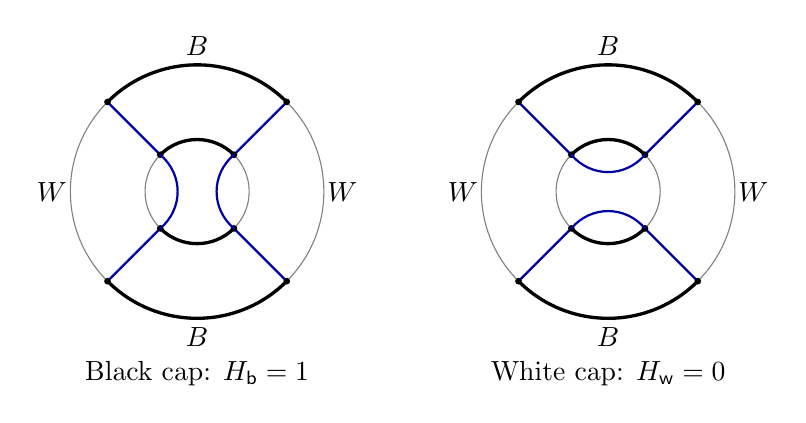
\begin{tikzpicture}[scale=0.87,line cap=round]
\foreach \a/\txt in {0/{Black cap: $H_{\mathsf b}=1$},6/{White cap: $H_{\mathsf w}=0$}} {
  \begin{scope}[xshift=\a cm]
    \draw[gray] (0,0) circle (1.85);
    \draw[gray] (0,0) circle (.76);
    \draw[very thick] (45:1.85) arc (45:135:1.85);
    \draw[very thick] (225:1.85) arc (225:315:1.85);
    \draw[very thick] (45:.76) arc (45:135:.76);
    \draw[very thick] (225:.76) arc (225:315:.76);
    \foreach \t in {45,135,225,315} {
      \draw[blue!65!black,thick] (\t:.76)--(\t:1.85);
      \fill (\t:.76) circle (1.4pt);
      \fill (\t:1.85) circle (1.4pt);
    }
    \node at (0,2.12) {$B$};
    \node at (0,-2.12) {$B$};
    \node at (-2.12,0) {$W$};
    \node at (2.12,0) {$W$};
    \node[align=center] at (0,-2.65) {\txt};
  \end{scope}
}
\draw[blue!65!black,thick] (45:.76) .. controls (.20,.25) and (.20,-.25) .. (315:.76);
\draw[blue!65!black,thick] (135:.76) .. controls (-.20,.25) and (-.20,-.25) .. (225:.76);
\begin{scope}[xshift=6cm]
\draw[blue!65!black,thick] (45:.76) .. controls (.25,.20) and (-.25,.20) .. (135:.76);
\draw[blue!65!black,thick] (225:.76) .. controls (-.25,-.20) and (.25,-.20) .. (315:.76);
\end{scope}
\end{tikzpicture}
\caption{The two cap pairings when all four walls are transmitted.
Blue curves are walls; thick black boundary arcs are black runs, and the
other runs are white.  The cap changes the outer black connection bit by
one.  The straight, unwound walls are schematic: the identity permits
winding and does not prescribe a pairing of numbered inner and outer
switches.}\label{fig:annular-caps}
\end{figure}

\subsection{The boundary convergence used below}

For $p>0$ let
\[
 \mathbb A_p=\{e^{-p}<|z|<1\}.
\]
Thus $p=\log(R/r)$ for a round annulus with radii $r<R$.  On both circles
angles increase counterclockwise.  Write $x=(x_1,x_2,x_3,x_4)$ for the outer
switches and $y=(y_1,y_2,y_3,y_4)$ for the inner switches, using increasing
lifts with $x_4<x_1+2\pi$ and $y_4<y_1+2\pi$.  Common translation of either
lift by $2\pi$ does not change the data.  The run following the first outer
switch is black.  For the $+$ prescription the corresponding inner run is
black; for the $-$ prescription it is white.

All limits in this section are taken along deterministic good sequences
of triangulations in the sense of \cite[Section 2, ``Deterministic
sequences and Jordan tests'']{V}.  In particular the mesh tends to zero on
compact sets, the joint Jordan-quad crossing limits hold, and the
mesh-first arm estimates recalled above are available.  Probabilities are
over product colors conditional on these triangulations.

\begin{definition}\label{an:admissible}
A sequence of marked graph annuli $D_n$ has \emph{admissible boundary
convergence} if it lies in a fixed bounded set and satisfies the following
conditions.
\begin{enumerate}
\item Each boundary is a simple site cycle.  With rotations normalized,
its uniformization
$\phi_n:\mathbb A_{p_n}\longrightarrow D_n$ extends continuously to the
closed annulus, where $p_n\to p\in(0,\infty)$.  After linear identification
in logarithmic radial coordinates, these maps converge uniformly on the
closed annulus to $\phi$.  The map $\phi$ is conformal and one-to-one in
$\mathbb A_p$, and its boundary traversal specifies the prime-end accesses
of $D=\phi(\mathbb A_p)$.
\item Each limiting boundary traversal is a concatenation of finitely
many simple arcs, each understood with its own access.  Different arcs
may meet in physical projection.  The two boundary components remain
distinct as prime-end boundary components.
\item The four switches on each component converge in these coordinates
to distinct switches.  Between them the prescribed run colors alternate.
The sites strictly between the two cycles have fresh independent fair colors.
\end{enumerate}
In graph constructions a boundary is taken without chords facing the
domain when that is required for a local boundary chart.  Such cuts are
obtained by the graph approximation and shortcut construction of
\cite[Section 2]{V}; at an exploration frontier, edges between already
revealed vertices are included before the frontier is taken.
\end{definition}

The definition permits a slit to have two different banks, even when
their images coincide.  It does not identify these banks.  The next
elementary convergence criterion explains how the domains arising from
stopped explorations fit this definition.

\begin{lemma}[A back with finitely many attached lobes]
\label{an:back-lobes}
Suppose graph annuli consist of an open annular back and finitely many
Jordan lobes attached to it along open seam intervals.  Assume that the
backs are Jordan annuli whose two complete boundary traversals converge
in curve order to those of a fixed Jordan annulus, the seam endpoints
converge in that order and the limiting seams remain open, and each lobe
converges as a Jordan domain with its boundary traversal.  The seam
incidences and cyclic order are fixed; lobes are glued only along their
specified seams, and their interiors are disjoint from the back and from
one another.  Suppose the resulting
limiting domain is an annulus, its hole and a separating open part of the
back persist, and the two boundary components stay physically apart.
Different limiting lobes may touch in projection but have disjoint
interiors.  Then the annular uniformizations converge uniformly on their
closures, with the stated accesses and traversal order.  In particular,
if the marked accesses converge and remain distinct, these domains have
admissible boundary convergence.
\end{lemma}

\begin{proof}
Every compact subset of a lobe persists by Jordan convergence.  The lobe
joins the back across every compact subinterval of its open seam.
Conversely, every point of the limiting boundary is approached by the
approximating boundaries.  Contacts between different lobes do not open
passages: the individual Jordan pieces are attached along their specified
seams, not through a point of contact.  These facts give kernel convergence
with the indicated accesses.  The persisting hole and separating back
exclude degeneration of the modulus.  The conformal kernel theorem
therefore gives convergence of normalized annular maps on interiors and
convergence of their moduli.

It remains to control the boundary parameters.  Fix a nonconstant open
subarc of one of the finitely many Jordan boundary pieces and a point in
the persisting back.  Jordan-map convergence in a lobe, or in a disk patch
along an unchanged back boundary, gives a positive lower bound for the
harmonic measure of a smaller subarc as seen from a point in that patch.
A Harnack chain through persisting interiors gives the same kind of lower
bound from the fixed back point.  In round annular coordinates the
harmonic-measure densities from its preimage are bounded above uniformly:
the moduli and the preimage stay in compact nondegenerate ranges.
Consequently no fixed nonconstant subarc of the boundary traversal can be
squeezed into an angular interval of length tending to zero.

The Jordan convergence of the finitely many pieces gives convergence of
the full boundary traversals in curve order.  Partition those traversals
into finitely many small image arcs, and apply the preceding lower bound
to intervening nonconstant subarcs.  A failure of equicontinuity in angular
parameters would traverse one such fixed subarc in a vanishing angular
interval, a contradiction.  This proves equicontinuity of the boundary
maps.  Interior convergence then identifies every uniformly convergent
subsequence, giving convergence on the closure.  Small crosscuts at the
finitely many joins give the same conclusion there.  There is no constant
boundary interval in the limiting conformal map, by uniqueness for a
holomorphic function continuous on a boundary arc.  The boundary order
and converging marked accesses thus also identify the limiting switches.
\end{proof}

\subsection{Boundary motion and annular crossing laws}

We first remove the rough banks.  The arm bounds needed here are
mesh-first statements: three free arms along one regular bank have an
upper bound with exponent $1+\eta$ for some $\eta>0$, and a free arm from a
shrinking neighborhood to a fixed scale has probability tending to zero.
The word \emph{free} excludes prescribed sites and cap wires.  The local
bank versions, including arms approaching the bank arbitrarily closely,
are those of \cite[Section 2, ``Cardy tests in a boundary chart'' and
``Free boundary-arm bounds'']{V}.

\begin{lemma}[Continuity under boundary motion]\label{an:motion}
For a sequence with admissible boundary convergence, move either cycle
slightly into the annulus in round coordinates, and move its switches
slightly with it.  Couple all unchanged free colors.  The probability
that either capped connection test changes tends to zero as the size of
the motion tends to zero, after taking the mesh limit.  The assertion also
holds for small piecewise smooth motions in spare space around an inset
annulus.  It is uniform along any convergent sequence of admissible data
with distinct limiting switches.  More precisely, if $H_n$ and
$H_{n,\delta}$ are either capped indicators before and after a motion of
size at most $\delta$, preserving the run order and its labels away from
the moving switches, then
\begin{equation}\label{an:motion-limit}
 \lim_{\delta\downarrow0}\limsup_{n\to\infty}
 \Pp(H_n\ne H_{n,\delta})=0.
\end{equation}
\end{lemma}

\begin{proof}
First the mesh in annular coordinates tends to zero.  Otherwise a
connected cell or triangle portion of vanishing physical diameter would
have preimages with a subsequential nontrivial continuum limit on which
$\phi$ is constant.  Such a continuum cannot meet the interior, where
$\phi$ is one-to-one, and cannot lie on the boundary, whose finitely many
simple arcs contain no constant interval.  Here graph portions, rather
than whole cells crossing the domain boundary, are used.

Remove small coordinate neighborhoods of the switches and of the
finitely many joins of simple bank arcs.  On each remaining compact bank
interval, use disk patches whose boundary consists of that bank and cuts
strictly inside the annulus.  Their physical boundaries are Jordan and
their graph approximations converge in curve order.  Their uniformizing
coordinates agree, with fixed-scale margins, with the annular coordinates;
reflection in the limiting round bank controls distortion on smaller
patches.  Thus the local boundary-arm estimates of \cite{V} apply on these
patches even when another prime-end bank has the same physical image.

Cover these intervals by $O(s^{-1})$ coordinate disks of radius $s$.
Implement a motion much smaller than $s$ by successively replacing bank
intervals, with tapered ends.  At graph level choose short transverse
joins in disjoint narrow strips from the old cycle to its replacement.
Substitute the intervals in cyclic order, retaining the old cycle off the
interval currently being changed and erasing the joins once the whole
cycle is replaced.  The graph approximation in curve order ensures that
these are simple cuts.  Each join has the same constant color as its run.
Moves containing switches or bank joins are instead included in the
exceptional neighborhoods.  Two nearby nonnested contours can be
compared through a common slightly inset contour.

Consider one ordinary move on a black bank.  If a capped connection test
changes, choose a winning black connection in one test and a winning
dual white connection in the other.  Contract the prescribed runs and
use the same cap in both tests.  Purely wired connections do not change,
so a free segment of a winning path must meet the support of the move.
The test neighborhood avoids every other run and mark.  The white path
has two free branches leaving that neighborhood.  At least one black
branch must also leave freely: a black branch already reaching the same
prescribed run outside the moved interval could be joined there without
the local change.  Taking simple paths after contraction gives disjoint
white branches, and the opposite-colored black branch is disjoint from
them in the common fair region.  This gives three free arms in a slightly
shifted half-patch, with fixed-factor margins.  The same argument applies
with the colors interchanged.  Forced sites on intermediate cuts are not
counted as free arms.

For any fixed larger chart scale, the mesh-first bound for a single disk
is $O(s^{1+\eta})$.  The union over $O(s^{-1})$ disks therefore costs
$O(s^\eta)$.  The number of exceptional neighborhoods is fixed.  A change
there requires a fair arm approaching from positive parameter distance:
connections already provided by the same run or by the cap do not
change.  This arm has positive physical diameter, uniformly after fixing
its outer parameter scale, by the no-continuum-fiber observation above.
The ordinary physical one-arm bound consequently makes the exceptional
cost tend to zero, including at a contact between different accesses.
One may move each exceptional neighborhood as a single piece, so this
cost is not multiplied by the number of ordinary intervals.

First take the mesh limit, then make the ordinary motions small compared
with $s$, then let $s$ tend to zero, and finally shrink the exceptional
neighborhoods.  This proves the assertion.  The same proof with moving
marks, or with a moving round radius, proves the stated continuity.
\end{proof}

After applying Lemma~\ref{an:motion}, all prescribed banks can be placed
on smooth contours strictly inside the parameter annulus, with spare
space on both sides.  There are still two separate issues: joint ordinary
crossings must have a conformally invariant annular law, and those
crossings must determine the capped tests.  We address them in that order.

\begin{lemma}[Ordinary crossings in an annular open set]
\label{an:ordinary}
In an annular open set compactly inside the parameter annulus, the joint
limiting law of any countable collection of regular ordinary quad tests
is conformally invariant.  The tests may be chosen from a countable dense
family of polygon or piecewise smooth quads with positive margins.
\end{lemma}

\begin{proof}
On every strict Jordan disk patch the joint law is the critical triangular
percolation law by \cite[Sections 3--4]{V}.  This law is conformally
invariant; see \cite[Theorems 1 and 7]{CN} and the quad-crossing
formulation in \cite[Section 2.3]{GPS}.  Scalar Cardy sandwiches identify smooth images of polygon
tests and nearby graph crossing conventions with the same limit.

Choose a finite-length smooth cut opening the annulus.  Any finite
collection of tests compactly contained off the cut fits in a strict
Jordan disk, so its joint law agrees in the physical domain and in the
conformal chart.  To recover tests meeting the cut, use the
Schramm--Smirnov gluing theorem
\cite[Theorem 1.19 and Proposition 4.1]{SS}, only in strict Jordan disk
patches.  For the critical triangular crossing law, the crossing of a
regular quad in such a patch is measurable, modulo null sets, with
respect to countably many tests avoiding the finite smooth cut in that
patch.  Its hypotheses hold here: independence in the discrete model,
RSW, one-arm decay, and a four-arm exponent strictly greater than one.
Regular continuity tests may be used throughout, by Cardy sandwiches.

Each required quad meeting the annular cut has a slightly larger Jordan
disk neighborhood inside the annulus.  The recovering measurable rule
in that neighborhood is the same in the chart and in its image, since
their whole disk laws already agree.  All recovering tests belong to the
common countable off-cut family.  Hence the recovered crossings have the
same joint law as well.  This proves the assertion.  White crossings are
included by Hex duality and continuity.  No gluing assertion along a rough
slit is used.
\end{proof}

\begin{proposition}[The annular transmission limit]\label{an:limit}
For every sequence with admissible boundary convergence, the probability
of $\mathcal T$ has a limit depending only on the round data $(p,x,y)$ and
the choice of inner colors.  Denote these limits by
\[
 T^+(p,x,y),\qquad T^-(p,x,y).
\]
They are continuous for $p>0$ and distinct switches.  The same convergence
holds for each capped connection probability.  In particular, it applies
to random remaining domains whenever, conditional on their geometry and
explored boundary, their interior colors are fresh and their marked
domains have admissible convergence almost surely in a subsequential
coupling.  In that case the difference between the conditional
transmission probability and $T^\pm$ evaluated at the actual annular
conformal data tends to zero in mean absolute value.
\end{proposition}

\begin{proof}
By Lemma~\ref{an:motion}, it suffices first to consider smooth inset
annuli with spare space.  We show that ordinary quad crossings determine
the limiting value of each capped black connection test.  Sample fair
colors throughout a slightly larger annular neighborhood in that spare
space, overriding them on prescribed runs only when evaluating a capped
test.  Ordinary tube tests use the fair colors.  Compare two
candidate sequences, one of which may be in round coordinates.  Couple
their countable ordinary crossing vectors through the common limiting
law of Lemma~\ref{an:ordinary}.  Along further subsequences include the
cap indicators in the coupling; the curve tightness proved below also
allows the chosen winning paths to be included.  The two limiting
collections are coupled to have the same ordinary crossing vector.

Fix a small \emph{favorable} perturbation of the black test in the second
sequence.  Move black banks into the annular fluid and extend their runs
slightly past the old switches; retreat white banks from the old fluid.
Use positive slacks and taper the motions within the old white
intervals, putting each new switch on the retreated part.  Thus every old
black attachment lies behind a new black bank, the new white banks are
positively separated from the old fluid, and any removed fluid is in
separate collars of the expanded black runs.  All these choices take
place in the spare space.

On a positive configuration in the first sequence, contract each
prescribed run and attach the cap edge when it is black.  Take an
outermost simple winning path between the two outer black terminals.
For example attach an external terminal edge and take the appropriate
boundary of the union of cycles containing it.  Contracting connected
boundary runs and attaching the cap preserves the planar embedding.
The resulting path has no bypass on its chosen exterior side.  Since it
visits each contracted run at most once, it decomposes into a bounded
number of free black segments joining different runs, together with
wired or cap joins.  Crop their endpoints by a vanishing graph distance
if they end adjacent to a wire.

We recall why these free segments admit simple limiting curves.  Many
oscillations across an annulus supply many disjoint free arms; BK and
one-arm decay bound their probabilities.  Successive-excursion
compactness therefore gives tightness in the curve metric.  A bulk
self-contact with two positive excursions would give four black
traversals.  In two gaps on the no-bypass side, intermediate transverse
cuts and Hex duality give two additional white traversals: a black
transverse crossing would instead be a bypass.  The six arms are
disjoint after fixed-factor crops, also for backtracking pieces.
The mesh-first six-arm exponent greater than two excludes such contacts
by a covering argument.  At a smooth boundary bank, a repeated visit to
the same point gives at least three free traversals, including when one
of the visits is an endpoint; the boundary exponent greater than one
excludes these repeated visits.  A single tangential bank contact need
not be excluded: the favorable perturbation accommodates it.  At the finitely
many switches one free arm suffices.  These are precisely the local
no-bypass and free-segment arguments of \cite[Section 4, ``Free segments
of a terminal path'']{V}.  Contracted runs do not change the bulk argument,
whose working annulus avoids them.  Constant pauses may be removed.

In a subsequential coupled representation, fix the favorable displacement
and then crop each limiting free segment a small positive amount at its
ends, keeping the new endpoints strictly behind the expanded black
banks.  A cropped endpoint may still lie on an old bank; the ambient
tube may straddle that bank within the spare space.  This positive crop is distinct from the vanishing
graph crop used to remove incidences to a wire.  Surround the cropped
simple segment by a thin Jordan tube, with end caps in those endpoint
neighborhoods.  The approximating free graph segments supply ordinary
fair-color crossings of this ambient tube.  The tube can be approximated with positive margins by a quad
from the countable ordinary test family.  Its crossing occurs in the
first sequence, and hence in the second for all sufficiently large
indices in the coupling.  The witnesses may be chosen from the countable
family after taking the subsequential limit; coordinatewise convergence
still applies to each of the finitely many chosen witnesses.

Clip these transferred crossings when they hit the new black banks.
Excursions outside the new fluid can only lie in the collars now wired
black.  They can be shorted through the corresponding run, and collars
of different black banks are separated.  This operation also handles
arbitrarily many backtracks: at graph level every passage between a
removed collar and the fluid meets its boundary cycle.  The transferred
tubes, together with the unchanged cap or wire joins, therefore give a
winning black connection in the favorably perturbed second test.

Apply this comparison to subsequences realizing the upper and lower
limits of the unperturbed cap probabilities.  The upper limit of the
first is bounded by the lower limit of the second plus its boundary-motion
error.  Remove the favorable perturbations using Lemma~\ref{an:motion}
and reverse the roles of the sequences.  Their upper and lower limits
coincide.  This proves convergence and conformal invariance of each cap
test on inset annuli.  Taking the inset size to zero proves the same
assertions under Definition~\ref{an:admissible}.  The cap identity gives
the transmission limit.  Allowing the marks and round radii to move in
the same comparison proves continuity in $(p,x,y)$.

Finally consider random remaining domains under the stated coupling.
For almost every convergent domain realization, the deterministic
statement applies to its fresh product-color law; continuity identifies
the same limit for $T^\pm$ at the actual conformal data.  All probabilities
are bounded by one, so bounded convergence gives convergence in mean
absolute value.  This conclusion does not assert a uniform conditional
estimate over arbitrary atypical explored boundaries.
\end{proof}

\begin{lemma}[Collisions and symmetries]\label{an:collision}
The functions $T^\pm$ extend continuously by zero when switches collide
on either boundary, uniformly for $p$ in compact subsets of $(0,\infty)$.
They are invariant under simultaneous rotation of $x$ and $y$ and under
global color reversal.  Cyclic relabeling by one switch in either tuple
interchanges $T^+$ and $T^-$.
\end{lemma}

\begin{proof}
\leavevmode\clubpenalty=10000
If two consecutive switches coalesce, four-interface transmission
requires a fair arm from their intervening shrinking run to the other
boundary.  This arm cannot use another prescribed run: it lies between
the two corresponding transmitted walls.  A mesh-first one-arm bound,
with a fixed outer scale and then a shrinking inner scale, proves
vanishing.  The bound does not depend on the positions of the other
switches and therefore also covers simultaneous collisions.
Conformal invariance gives simultaneous rotational invariance, and
fair colors give global color symmetry.  Moving the first switch to the
next switch reverses the alternating run labels on that component.
By the defining convention, this interchanges the two inner prescriptions.
\end{proof}

\section{The spectrum of four-interface transmission}
\label{sp:section}
\label{sec:spectrum}

We now estimate the limiting transmission probabilities
$T^\pm(p,x,y)$ of Section~\ref{sec:annuli} when the modulus $p$ is large.
There are two different conclusions.  The leading term separates into an
inner factor and an outer factor.  The signed difference $T^+-T^-$ has
additional decay, and averaging the rotation of one end improves that
decay beyond exponent $2$.  This last improvement will make the response
to a fair Poisson insertion integrable over the plane.

\subsection{The modulus equation}

The space of four cyclically ordered, labeled angles is
\[
 \mathcal C=
 \{w\in\R^4:w_1<w_2<w_3<w_4<w_1+2\pi\}
       /(2\pi\mathbb Z\mathbf 1).
\]
Thus we quotient by simultaneous full turns, not by cyclic relabeling.
We use the product chamber $\mathcal X=\mathcal C\times\mathcal C$ for
$(x,y)$.  All statements about distances or derivatives on this chamber
use local angle lifts.  Constants are uniform as angles approach a
collision; moduli are bounded below by a fixed positive constant.

\begin{proposition}[Modulus equation]\label{sp:annular-pde}
The functions $T^\pm$ are smooth on $(0,\infty)\times\mathcal X$ and
satisfy
\begin{equation}\label{sp:pde}
 \partial_pT=(L+B_p\cdot\nabla)T,
 \qquad
 L=\frac18\sum_{w=x,y}
 \left(3\sum_{i=1}^4\partial_{w_iw_i}
 +\sum_{i=1}^4\sum_{j\ne i}
       \cot\frac{w_i-w_j}{2}\,\partial_{w_i}\right).
\end{equation}
For every $p_0>0$ and every fixed finite derivative order $k$,
the vector field $B_p$ extends smoothly across angle collisions and
\[
 \|B_p\|_{C^k}\le C_{k,p_0}e^{-p}\qquad(p\ge p_0).
\]
It is equivariant under permutations within either tuple, common
rotations, and cyclic relabelings.  In particular, its normal component
at every collision face is zero.
\end{proposition}

\begin{proof}
We first derive a local equation with just one switch active.  Write the
annulus as the cylinder $0<\operatorname{Im}z<p$, with real period
$2\pi$, and take the active switch on its lower boundary.  Parametrize
its exploration by the decrease of the modulus.  In the annulus Loewner
normalization with zero regular constant at the driving pole, the
angular kernel is
\[
 H_p(u)=\lim_{N\to\infty}\sum_{k=-N}^N
                     \cot\frac{u-2ikp}{2}.
\]
The pole has residue $2$, and the imaginary part on the other boundary
is $-1$.  The locality theorem for annulus $\mathrm{SLE}_6$
\cite{Zhan} identifies the local driving angle with Brownian motion
of variance parameter $6$.  Only locality before leaving a small
simply connected neighborhood of the active switch is used here.

For completeness, the absence of an additional driving drift depends
on the normalization.  In a chordal chart the pole part is
$2/(z-U_t)$.  If $F_t$ is a changing local conformal coordinate, comparison
of pole residues gives the new clock $F_t'(U_t)^2\,dt$.  Comparison of
the regular terms, both normalized to have zero constant, gives
$\partial_tF_t(U_t)=-3F_t''(U_t)$.  This cancels the It\^o correction
$\kappa F_t''(U_t)/2$ precisely for $\kappa=6$.
No condition on a remote target in the annulus enters this calculation.

Other switches on the active boundary have velocity $H_p(u)$, at
angular difference $u$ from the active one.  Switches on the opposite
boundary have angular velocity $\operatorname{Re}H_p(u+ip)$.
Pairing the positive and negative terms of the series gives, uniformly
with any fixed number of derivatives,
\begin{equation}\label{sp:kernel-errors}
 H_p(u)-\cot(u/2)=O(e^{-2p}),
 \qquad \operatorname{Re}H_p(u+ip)=O(e^{-p}).
\end{equation}
The remainders are smooth periodic functions of $u$, including at
$u=0$.  Thus, when $x_i$ is the active switch, its equation is
\begin{equation}\label{sp:active-equation}
 \begin{aligned}
 0={}&-\partial_pT+3\partial_{x_ix_i}T
       +\sum_{j\ne i}H_p(x_j-x_i)\,\partial_{x_j}T\\
    &+\sum_{j=1}^4\operatorname{Re}H_p(y_j-x_i+ip)\,
                                      \partial_{y_j}T.
 \end{aligned}
\end{equation}
For an active switch $y_i$, the equation is obtained by exchanging
$x$ and $y$.  Indeed the cylinder change $z\mapsto-z+ip$ exchanges
the boundaries and reverses both angle coordinates; the angular
kernels are odd, so transforming back preserves the displayed signs.
Averaging these eight equations gives \eqref{sp:pde}.
The series estimates give the asserted bounds on $B_p$.  The averaged
expression treats the labels within each tuple symmetrically; therefore
it is permutation equivariant.  At a collision its two corresponding
components agree, proving tangency.  The other symmetries follow in
the same way from the kernels.

We justify the Markov identity underlying these equations before
assuming differentiability.  On a round annulus choose an arbitrarily
small crosscut around the active switch, separated from all other
switches and from the other boundary component.  Approximate the smooth
bank by chord-free graph boundaries and complete the neighborhood to a
Jordan patch, putting its second color switch remotely.  Up to the
pre-query stop at the crosscut, the exploration in this patch is exactly
the exploration in the annulus: no color beyond the crosscut is read.
The stopped-exploration results of \cite[Lemmas~3.6--3.7]{V} give convergence
of the path together with its remaining domains.  Crosscuts may be
chosen as the semicircle crosscuts in the stopped-target construction;
the probability of an endpoint stop vanishes when endpoint
neighborhoods shrink.

The unaltered part, obtained by cutting off the fixed crosscut
neighborhood, is a Jordan annular back with unchanged boundary
traversal.  For the remaining face containing this back, the stopped-target-face
and remaining-domain statements of \cite[Lemmas~3.6--3.7]{V}
give finitely many Jordan side pieces attached to the back along
open subintervals of that crosscut.  Components already disconnected
from this face are discarded; no assertion of finiteness is being
made about all components swallowed by the exploration.
We check that its limit is still doubly connected.  In the closed
crosscut neighborhood, remove the side-lobe interiors and their open
attaching intervals.  The remaining closed set is connected to the
original outer complement.  Indeed join any of its points to the old
outer bank by a path in that neighborhood whose interior avoids the
crosscut.  If this path enters a lobe, replace its portion from first
entry to last exit by the corresponding subarc of the lobe boundary
off its open attachment.  The entry and exit lie on this retained
bank, not on the crosscut.  This bank meets the crosscut only at its
own endpoints and enters no other lobe interior, since the Jordan
interiors are disjoint.  Thus each replacement avoids all lobe
interiors and open attachments; finitely many replacements give a
path in the complement.  The unchanged inner hole is separated from
this connected outer complement by the persisting annular back.
These are precisely the two nondegenerate complementary components.
Lemma~\ref{an:back-lobes} gives convergence of annular uniformizations
on their closures, with the prime-end traversals and marks in order.
The hole and a separating open bulk persist throughout this local
exploration, so the moduli remain nondegenerate.  Thus the residual
annuli satisfy the hypotheses of Proposition~\ref{an:limit}.  The stopping
edge becomes the replacement switch, the other marks are unchanged,
and the colors in the remaining face are fresh.  Transmission topology
and bounded convergence therefore give the local mean-value identity
for $T^\pm$ at each of these hull stops.

This identity first implies the active equations in the viscosity
sense.  Work modulo simultaneous rotation and let a smooth test
function touch $T$ from above or below.  On a sufficiently small
crosscut stop the modulus and image marks remain in the touching
neighborhood.  Indeed the hull capacity tends to zero, and annular
maps normalized at a remote mark tend to the identity on the other
compact bank intervals, by reflection.  The image of the tip is
squeezed between neighboring unaffected bank points.  Applying It\^o's
formula to the touching function contradicts a strict inequality with
the wrong sign in the active equation, because the stop takes positive
time.  The same touching function can be used for all eight active
equations, so their average also holds in viscosity form.  On every
compact subset of the open chamber the averaged equation is a smooth,
uniformly parabolic linear equation, also after the rotation quotient.
Interior parabolic regularity then gives smoothness and the classical
equation.  Simultaneous rotation invariance removes the quotient.
\end{proof}

\subsection{The ground-state transform}

Define positive functions on the open chamber by
\begin{equation}\label{sp:ground-state}
 J(w)=\prod_{1\le i<j\le4}\sin\frac{w_j-w_i}{2},\qquad
 h(x,y)=J(x)^{1/3}J(y)^{1/3},\qquad \lambda=\frac54.
\end{equation}
The product $J$ is unchanged by a cyclic relabeling.  For one tuple put
$s_i=\sum_{j\ne i}\cot((w_i-w_j)/2)$.  The elementary three-angle
cotangent identity gives
\[
 \sum_i s_i^2=\sum_{i\ne j}\csc^2\frac{w_i-w_j}{2}-20,
 \qquad \partial_{w_i}\log J^{1/3}=\frac{s_i}{6}.
\]
Substitution in $L$ shows that each tuple contributes $-5/8$ to
$h^{-1}Lh$.  Hence $Lh=-\lambda h$.

This ground-state calculation is the cotangent-diffusion form of the
SLE--Calogero--Sutherland structure studied in \cite{CardyCS}; we give
the estimates needed here directly.  The transformed generator and
its invariant density are
\begin{equation}\label{sp:doob-generator}
 D=\frac38\bigl(\Delta+\nabla\log m\cdot\nabla\bigr),
 \qquad m(x,y)=J(x)^{4/3}J(y)^{4/3}.
\end{equation}
Let $\mu$ be the probability measure proportional to $m$ times Lebesgue
angle measure.  For $T=T^+,T^-$, or a linear combination of them, set
$W(p)=e^{\lambda p}T(p)/h$.  Equation~\eqref{sp:pde} becomes
\begin{equation}\label{sp:transformed-pde}
 \partial_pW=DW+B_p\cdot\nabla W+V_pW,
 \qquad V_p=B_p\cdot\nabla\log h.
\end{equation}
The apparent singularities of $V_p$ at collisions are removable.
Every cotangent is multiplied by a difference of two components of
$B_p$, which vanishes on the corresponding collision face.
Periodicity handles the face $w_4=w_1+2\pi$.  Thus $V_p$ has smooth
bounds $O(e^{-p})$ up to the chamber boundary, as does $B_p$.

\begin{lemma}[Smoothing on the chamber]\label{sp:smoothing}
Fix $p_0>0$.  For either transmission function, or its sum or difference,
the transformed solution satisfies
\begin{equation}\label{sp:uniform-smoothing}
 \|W(p)\|_\infty+\operatorname{Lip}(W(p))\le C_{p_0}
 \qquad(p\ge p_0+2).
\end{equation}
The semigroup $P_t$ of $D$ is symmetric on $L^2(\mu)$ and, for every
$q>1$, maps $L^q(\mu)$ to bounded functions at every fixed positive
time.  At unit time the evolution in \eqref{sp:transformed-pde} maps
bounded functions to Lipschitz functions with a constant uniform in
the starting modulus $p\ge p_0$.
\end{lemma}

\begin{proof}
We first justify using the diffusion all the way to the chamber
boundary.  The drift in one tuple is
$\frac14(\sum_{j\ne i}\cot((w_i-w_j)/2))_{i=1}^4$.
On the lifted convex chamber, use $-\log m$, shifted to be nonnegative,
as a Lyapunov function.  If $\alpha=4/3$ is the density exponent, the
cotangent identity shows that its generator has a singular contribution
proportional to $(\alpha-\alpha^2)\sum_{i<j}\csc^2((w_i-w_j)/2)$.
This coefficient is negative, so the generator is bounded above.
More explicitly, the one-tuple contribution is
\[
 D(-\log J^{4/3})=
 \frac{10}{3}-\frac1{24}\sum_{i\ne j}
                           \csc^2\frac{w_i-w_j}{2}.
\]
Stopping on inner exhaustions proves that no collision occurs in
finite time.  Interior existence and pathwise uniqueness therefore
give a global diffusion.  A bounded added drift, such as the
time-dependent $B_p$, preserves noncollision by Girsanov's theorem on
each bounded time interval.  The divergence form of $D$ gives symmetry
and invariance of $\mu$, first on interior exhaustions and then by
noncollision.

The Feynman--Kac representation for
\eqref{sp:transformed-pde} uses $D+B\cdot\nabla$ and potential $V$,
with coefficients read at decreasing moduli from the evaluation
modulus down to the initial modulus.  Its initial data at $p_0$ obey
$|W(p_0)|\le C/h$.  To justify this representation despite the
unbounded transformed data, first apply the killed representation to
$T$ on inner chamber exhaustions.  Lemma~\ref{an:collision} says that
the lateral values of $T$ tend uniformly to zero on each compact
modulus interval.  Their contribution therefore disappears.
The $h$-transform on the exhaustion gives the stated representation;
pass to the limit using noncollision.  It suffices to do this for the
nonnegative $T^\pm$ and then use linearity.

Here are the uniform smoothing estimates.  The negative logarithm of
$m$ is convex on the lifted chamber, so the drift of $D$ is monotone
dissipative.  Couple two diffusions by the same Brownian motion and
add to the second a drift toward the first of magnitude their initial
distance divided by the allotted time, until they meet.  Dissipativity
forces meeting by that time.  Girsanov's theorem removes the extra
drift with all fixed moments bounded in terms of the time and the
initial distance.  Localization inside the chamber justifies the
coupling, and the preceding change-of-measure argument excludes
collisions for the controlled diffusion.  H\"older's inequality gives
the dimension-free form
\[
 |P_tF(z)|^q\le
 C(q,t,\operatorname{dist}(z,z'))P_t(|F|^q)(z').
\]
One can always choose lifts of $z,z'$ at bounded distance.
Integration in $z'$ against the invariant probability $\mu$ proves
the asserted $L^q$-to-supremum estimate.

A bounded drift perturbation and a bounded potential on a unit time
interval preserve initial smoothing from $L^4(\mu)$.
Indeed Cauchy--Schwarz applied to the Girsanov density bounds the
perturbed expectation of $|f|$ by $C(P_1|f|^2)^{1/2}$;
the unperturbed $L^2$-to-supremum bound for $|f|^2$ then gives
$C\|f\|_{L^4(\mu)}$.  There is exactly this integrability here:
$h^{-1}\in L^4(\mu)$, since $h^{-4}m=1$.
After the first unit interval $W$ is bounded.  Its bound persists
for all subsequent times because
$\int_{p_0}^\infty\|V_p\|_\infty\,dp<\infty$.

The same coupling proves a Lipschitz estimate for bounded data on a
unit interval.  In the presence of $B$, a control of size at most a
fixed constant times the initial distance forces meeting; before
meeting the distance stays bounded by the same multiple of the
initial distance.  The second moment estimate for the Girsanov
exponential bounds its total-variation cost by that distance.
The two Feynman--Kac weights differ by at most the same order, since
$V$ has a uniform Lipschitz bound.  Thus the unit-time Lipschitz norm
is bounded by a constant times the initial supremum norm.  Apply this
on the last unit interval to obtain
\eqref{sp:uniform-smoothing}.
\end{proof}

\subsection{The two symmetry gaps}

The role of rotation averaging can now be seen explicitly.  For a
tuple with real ordered lift $w$, write
\[
 \bar w=\frac14\sum_iw_i,\qquad
 r=w-\bar w\mathbf1,\qquad \theta=\bar w\pmod{2\pi}.
\]
The relative coordinate lies in the bounded convex alcove
\[
 \mathcal A=\{r\in\R^4:\textstyle\sum_ir_i=0,
                         \ r_1<r_2<r_3<r_4<r_1+2\pi\}.
\]
This identifies $\mathcal C$ with a product of a circle and
$\mathcal A$.  Its invariant law is a product as well, since $J$
depends only on the relative angles.  The center part of $D$ is
$(3/32)\partial_\theta^2$ for each tuple.

\begin{lemma}[Spectral gaps]\label{sp:gaps}
The relative-angle diffusion for one tuple has Poincar\'e gap at least
$1/2$.  Consider the subspace of $L^2(\mu)$ consisting of functions
invariant under simultaneous rotation of the two tuples and changing
sign under one cyclic relabeling of either tuple.  On this subspace
$-D$ has gap at least $3/4$.  On its subspace with both center
frequencies zero the gap is at least $1$.
\end{lemma}

\begin{proof}
For a mean-zero vector $v\in\R^4$ the Hessian of the negative
logarithm of the one-tuple density satisfies
\[
 \nabla^2(-\log J^{4/3})[v,v]
 =\frac13\sum_{i<j}\csc^2\frac{r_i-r_j}{2}(v_i-v_j)^2
 \ge\frac43|v|^2.
\]
The Brascamp--Lieb inequality \cite{BL,KM}, applied on the convex alcove,
therefore gives
\[
 \operatorname{Var}(F)\le\frac34\int|\nabla_rF|^2\,d\mu_r.
\]
The Dirichlet form has factor $3/8$, yielding the gap $1/2$.
One may first use inner convex exhaustions of the alcove and then
pass to the limit.

For the two tuples, simultaneous rotation invariance allows only
center frequencies $(n,-n)$, whose energy cost is $3n^2/16$.
A cyclic relabeling sends $\theta$ to $\theta+\pi/2$ and acts on
$\mathcal A$ by a measure-preserving affine isometry.  If a function
changes sign under this relabeling, its relative-angle mean must
vanish unless $e^{in\pi/2}=-1$, that is, unless $n\equiv2\pmod4$.
The same assertion holds separately for the other tuple.  Therefore
frequencies not congruent to $2$ modulo $4$ pay at least $1/2+1/2=1$
in relative energy.  The remaining frequencies have $|n|\ge2$ and
pay at least $3/4$ in center energy.  At $(n,-n)=(0,0)$ the two
relative means vanish, giving the gap $1$.

These inequalities give $L^2$ semigroup decay through the symmetric
Dirichlet form
\[
 \mathcal E(F,F)=\frac38\int|\nabla F|^2\,d\mu.
\]
There is no hidden absorbing boundary: the constant function is in
the form domain.  Cutoffs approaching the collision faces have
vanishing energy because the density vanishes with power $4/3>1$.
\end{proof}

Let $W_-=e^{\lambda p}(T^+-T^-)/h$, and define
\[
 (\Pi F)(x,y)=\frac1{2\pi}\int_0^{2\pi}
                           F(x,y+\phi\mathbf1)\,d\phi
\]
on simultaneous-rotation-invariant functions.  Equivalently, $\Pi$
is projection to center frequencies $(0,0)$.  A one-step cyclic
relabeling switches $T^+$ and $T^-$, while $h$ is unchanged.
Thus $W_-$ has exactly the symmetries of Lemma~\ref{sp:gaps}.

\begin{proposition}[Uniform transmission asymptotics]
\label{sp:transmission-asymptotics}
There are constants $K\ge0$, $\sigma>0$, and $C<\infty$ such that,
uniformly over the open angle chamber and all sufficiently large $p$,
\begin{align}
 \|W_-(p)\|_\infty&\le Ce^{-3p/4},
 &\|\Pi W_-(p)\|_\infty&\le C(1+p)e^{-p},
 \label{sp:odd-decay}\\
 T^\pm(p,x,y)&=e^{-\lambda p}
                   \bigl(Kh(x,y)+O(e^{-\sigma p})\bigr).
 \label{sp:rank-one-round}
\end{align}
Moreover,
\begin{equation}\label{sp:odd-regularity}
 \operatorname{Lip}(W_-(p))\le Ce^{-3p/4},\qquad
 \|W_-(p+\ell)-W_-(p)\|_\infty
        \le Ce^{-3p/4}\sqrt\ell\quad(0\le\ell\le1).
\end{equation}
The function $h$ is uniformly $1/3$-H\"older on the closed chamber.
\end{proposition}

\begin{proof}
For any transformed solution put
$F_p=B_p\cdot\nabla W(p)+V_pW(p)$.
Lemma~\ref{sp:smoothing} implies $\|F_p\|_\infty\le Ce^{-p}$
once $p$ is sufficiently large.  Variation of constants gives
\begin{equation}\label{sp:duhamel}
 W(p)=P_{p-p_1}W(p_1)+\int_{p_1}^pP_{p-s}F_s\,ds.
\end{equation}
This identity also follows directly by It\^o's formula with $D$,
first stopping on inner exhaustions: on the interval in question
the solution and the forcing are bounded, and collisions are not hit.

For $W_-$ the forcing respects simultaneous rotation invariance and
the two cyclic sign changes.  Apply the $3/4$ gap to
\eqref{sp:duhamel}, and then apply the unit-time $L^2$-to-supremum
smoothing to all semigroup times at least one.  For shorter times
use the supremum bound on $F_s$.  The convolution with $e^{-s}$ is
$O(e^{-3p/4})$.  After projecting by $\Pi$, which commutes with $D$,
the gap is $1$ and the convolution is $O((1+p)e^{-p})$.
This proves \eqref{sp:odd-decay}.  It does not require $B_p$ to
commute with independent rotations: the projected forcing is
estimated after projection.

For either $W^+$ or $W^-$ separately, $D$ has a positive gap off
constants.  Indeed the center gap is $3/32$ and the relative gap is
at least $1/2$.  The same argument shows exponential convergence of
$W-\int W\,d\mu$ to zero.  Also
$\partial_p\int W\,d\mu=\int F_p\,d\mu=O(e^{-p})$, so its mean
converges exponentially.  The first estimate of
\eqref{sp:odd-decay} makes the two limiting constants equal; call
their common value $K$.  Multiplication by $e^{-\lambda p}h$
proves \eqref{sp:rank-one-round}.

The unit-interval Lipschitz estimate in Lemma~\ref{sp:smoothing},
applied to the homogeneous perturbed evolution for $W_-$, improves
its Lipschitz bound to $Ce^{-3p/4}$.  To obtain time regularity,
the same diffusion has expected angle displacement at most
$C\sqrt\ell$ in time $\ell\le1$, uniformly in its initial point.
Here is a bound that remains valid near a collision.  Apply It\^o's
formula to squared distance from the initial lift.  Each pair in
the scalar product with the singular drift contributes a constant
multiple of
\[
 (v-v_0)\cot(v/2),\qquad v,v_0\in(0,2\pi),
\]
which is bounded above uniformly: use $v-v_0\le v$ for $v\le\pi$
and $v-v_0\ge v-2\pi$ for $v\ge\pi$.
The bounded additional drift and the Brownian quadratic variation
then give $\E|Z_\ell-Z_0|^2\le C\ell$, by localization and
Gronwall's inequality.  The Feynman--Kac representation over time
$\ell$, the spatial Lipschitz bound, and the bounded potential give
the time estimate in \eqref{sp:odd-regularity}.
Finally $J$ is a bounded Lipschitz nonnegative function on the closed
chamber, and taking a cube root is $1/3$-H\"older.  The assertion
for $h$ follows by taking products.
\end{proof}

\section{Separating the conformal data of the two ends}
\label{sh:section}
\label{sec:shape}

The estimates of Section~\ref{sp:section} are expressed in the
uniformizing coordinates of the entire annulus.  To use them in a
transfer operator, their leading term must instead depend separately
on the inner and outer explored regions.  We prove the requisite
comparison uniformly over their shapes.  Only separation of the
two ends is needed; no boundary smoothness bound is imposed.

Let $K_i$ be a closed Jordan region containing $0$ in its interior,
and let $U_o$ be a bounded Jordan domain containing $K_i$.
The annulus under consideration is $U_o\setminus K_i$.
Fix constants $c_*,C_*>0$ and assume that
\begin{equation}\label{sh:shape-hypotheses}
 K_i\subset\{|z|\le a\},\quad
 \operatorname{diam}K_i\ge c_*a,\qquad
 \{|z|<b\}\subset U_o,\quad
 \min_{z\in\partial U_o}|z|\le C_*b.
\end{equation}
We take $b/a$ larger than a constant depending only on $c_*,C_*$.
Each boundary carries four distinct marked prime ends and alternating
color prescriptions.

Normalize the two ends separately.  Let
\[
 w_i:\widehat\C\setminus K_i\longrightarrow\{|w|>1\},
 \qquad w_i(z)=z/l_i+O(1)\quad(z\to\infty),
\]
with $l_i>0$, and let
\[
 w_o:U_o\longrightarrow\{|w|<1\},\qquad
 w_o(0)=0,\quad w_o'(0)=1/l_o>0.
\]
Thus $l_i$ is the logarithmic capacity of $K_i$ and $l_o$ is the
conformal radius of $U_o$ at $0$.  Write $y^0,x^0$ for the angles of
the inner and outer marks in these maps.  Capacity-diameter bounds
for continua and the Koebe estimates imply
\begin{equation}\label{sh:end-scales}
 l_i\asymp a,\qquad l_o\asymp b,
\end{equation}
with constants depending only on $c_*,C_*$.

\begin{lemma}[Uniform end-map comparison]\label{sh:comparison}
Let $(p,x,y)$ be the modulus and marked angles in a uniformization
of $U_o\setminus K_i$, with angular direction the same on both
boundary components.  Put $p'=\log(l_o/l_i)$.  The common rotational
normalization of the annulus map can be chosen so that
\begin{equation}\label{sh:comparison-estimate}
 |p-p'|\le C\frac ab,\qquad
 |x-x^0|+|y-y^0|
       \le C\bigl(1+\log(b/a)\bigr)\frac ab.
\end{equation}
Distances in the second inequality use compatible cyclic lifts.
The constant is uniform over all Jordan boundaries satisfying
\eqref{sh:shape-hypotheses}, including all placements of the marks.
\end{lemma}

\begin{proof}
Define the single-valued analytic corrections
\[
 g_i(z)=\log\frac{l_iw_i(z)}z,
 \qquad g_o(z)=\log\frac{l_ow_o(z)}z,
\]
with branches vanishing at infinity and at zero, respectively.
The quotient defining $g_o$ has no zeros in $U_o$ and the apparent
singularity at zero is removable; the exterior quotient has zero
winding and its logarithm is normalized at infinity.
Univalent distortion and \eqref{sh:end-scales} give
\begin{equation}\label{sh:correction-bounds}
 |g_o(z)|\le Ca/b\quad (|z|\le C_1a),\qquad
 |g_i(z)|\le Ca/b\quad (|z|\ge c_1b),
\end{equation}
for every fixed $C_1<\infty$ and $c_1>0$, once $a/b$ is small
enough.  The relevant sets in these inequalities are contained in
the respective map domains.  The same bounds hold in fixed round
collars in the single-end coordinates.  If $\psi_i=w_i^{-1}$,
the maximum principle applied to $\psi_i(w)/w$ gives
$|\psi_i(w)|\le a|w|$ for $|w|>1$.
For $\psi_o=w_o^{-1}$, Koebe's distortion bound gives
$|\psi_o(w)|\ge l_o|w|/(1+|w|)^2$.
Thus the inverse exterior map sends $1\le|w_i|\le2$ into
$|z|\le2a$, and the inverse interior map sends, for example,
$1/2\le|w_o|<1$ into $|z|\ge cb$.
These observations are the reason arbitrary roughness of the physical
boundaries does not change the constants.

Consider the multivalued analytic function
\[
 H(z)=\log(z/l_i)+g_i(z)+g_o(z).
\]
It has period $2\pi i$, and its real part is within $Ca/b$ of $0$
on the inner boundary and of $p'$ on the outer boundary.  Let
$A(z)$ be an annulus logarithm, normalized by
$0<\operatorname{Re}A<p$.  Its period is also $2\pi i$.
The difference $H-A$ is therefore single-valued.  In the cylinder
coordinate $A$, the circular average of the real part of any
single-valued analytic function is constant across the cylinder.
At the two boundary circles the averages of
$\operatorname{Re}(H-A)$ are, respectively, $O(a/b)$ and
$p'-p+O(a/b)$.  Equality of the averages proves
$|p-p'|\le Ca/b$.  The maximum principle now yields
\begin{equation}\label{sh:real-error}
 |\operatorname{Re}(A-H)|\le Ca/b
 \quad\hbox{throughout }U_o\setminus K_i.
\end{equation}

It remains to compare the angular parts; a bound on real parts
alone would not control them on arbitrary boundaries.  Use instead
the round collars in the single-end coordinates.  The relevant
single-valued functions satisfy
\[
 A-\log w_i=(A-H)+g_o,\qquad
 A-p-\log w_o=(A-H)+(p'-p)+g_i.
\]
Near the inner
end, $A-\log w_i$ has real part bounded by $Ca/b$, by
\eqref{sh:correction-bounds} and \eqref{sh:real-error}, and its
real part is exactly zero on $|w_i|=1$.  Schwarz reflection across
this circle, followed by interior gradient bounds on a smaller fixed
collar, bounds the variation of its imaginary part along the entire
end circle by $Ca/b$.  Near the outer end apply the same argument
to $A-p-\log w_o$.  Its real part is zero on $|w_o|=1$ and is
bounded by $Ca/b$ in a fixed inner collar.  This gives the analogous
angular bound, initially with possibly different additive constants
at the two ends.

To match these constants, choose $C_1$ large and $c_1$ small, both
fixed.  The round annulus $C_1a<|z|<c_1b$ is contained in the
physical annulus.  Along a radial segment across it, use
$O(1+\log(b/a))$ overlapping disks of fixed relative size.
The gradient estimate for the analytic function $A-H$, whose real
part obeys \eqref{sh:real-error}, bounds the variation of its
imaginary part on each disk by $Ca/b$.
At either end, distortion in the corresponding single-end chart
connects this radial segment to the fixed collar with a bounded
additional chart distance.  The same interior estimate and the
collar reflection estimate apply there.
Thus the two additive constants differ by at most
$C(1+\log(b/a))a/b$.  Choose the common rotation to fix the inner
constant.  The comparison of all marked angles, uniformly even
when marks are very close, follows.  This proves
\eqref{sh:comparison-estimate}.
\end{proof}

\begin{proposition}[Separated-end transmission]\label{sh:separated-ends}
There are constants $\sigma_1,\sigma_2>0$ and $C<\infty$,
depending only on the fixed constants in
\eqref{sh:shape-hypotheses}, such that the transmission probabilities
of every such marked annulus satisfy
\begin{equation}\label{sh:rank-one}
 \left|T^\pm-
 K\,l_i^\lambda J(y^0)^{1/3}\,
       l_o^{-\lambda}J(x^0)^{1/3}\right|
 \le C(a/b)^{\lambda+\sigma_1}.
\end{equation}
Here $K$ is the common constant in
Proposition~\ref{sp:transmission-asymptotics}.  If one rotates the
inner end, with its marks and prescribed colors, through angle $\phi$
about $0$ while keeping the outer end fixed, then
\begin{equation}\label{sh:rotation-average}
 \left|\frac1{2\pi}\int_0^{2\pi}
                 \bigl(T^+_\phi-T^-_\phi\bigr)\,d\phi\right|
       \le C(a/b)^{2+\sigma_2}.
\end{equation}
The same conclusion holds if the outer end is rotated instead.
Both estimates remain uniform for Jordan approximants to the
prime-end boundaries of Section~\ref{sec:annuli}, provided they
satisfy \eqref{sh:shape-hypotheses} with the same fixed constants.
\end{proposition}

\begin{proof}
Write $\rho=a/b$ and $q=\log(1/\rho)$.  By
\eqref{sh:end-scales}, $p'=q+O(1)$.  Set
$\eta=C(1+q)\rho$, the angular error in
Lemma~\ref{sh:comparison}.  The $1/3$-H\"older bound for $h$
and the first inequality of that lemma give
\[
 |e^{-\lambda p}h(x,y)-e^{-\lambda p'}h(x^0,y^0)|
       \le C\rho^\lambda(\rho+\eta^{1/3}).
\]
Combining this with \eqref{sp:rank-one-round} proves
\eqref{sh:rank-one}; for example any
$0<\sigma_1<\min\{\sigma,1/3\}$ is sufficient after changing
the constant.  Since
$e^{-\lambda p'}=(l_i/l_o)^\lambda$, the leading term has exactly
the displayed separated form.

For the signed estimate put $U=T^+-T^-=e^{-\lambda p}hW_-$.
Equations~\eqref{sp:odd-decay} and
\eqref{sp:odd-regularity}, together with the H\"older bound for
$h$, show that replacing the actual annular data by the two
single-end data costs at most
\begin{equation}\label{sh:signed-shape-error}
 C\rho^2\bigl(\rho^{1/2}+\eta+\eta^{1/3}\bigr).
\end{equation}
This bound is uniform over the rotation of either physical end.
In particular it is a power improvement on $\rho^2$.

The capacity $l_i$ is unchanged by rotation of the inner end, and
its normalized map is
$w_{i,\phi}(z)=e^{i\phi}w_i(e^{-i\phi}z)$.
Consequently its marked single-end angles are exactly
$y^0+\phi\mathbf1$.  The factor $h$ is unchanged by rotating
either tuple separately.  Thus the rotation average in the unperturbed
data is
\[
 e^{-\lambda p'}h(x^0,y^0)
                       (\Pi W_-)(p',x^0,y^0),
\]
whose absolute value is at most
$C(1+q)\rho^{\lambda+1}=C(1+q)\rho^{9/4}$ by
\eqref{sp:odd-decay}.  Add the uniform error
\eqref{sh:signed-shape-error}.
Any $0<\sigma_2<1/4$ is then admissible, after increasing the
constant and restricting to sufficiently small $\rho$.
Rotating the outer end gives the same projection, by simultaneous
rotation invariance.

Every estimate was obtained with constants depending only on the
separation and scale conditions, not on boundary smoothness or mark
separation.  It can therefore be applied directly to the continuum
function $T$ evaluated on the conformal data of the Jordan cycles
approximating an explored domain.  Under admissible convergence,
Proposition~\ref{an:limit} separately identifies the limit of the
discrete transmission probabilities with that continuum function; no
reflection across a physically nonsimple limiting bank is being
asserted.
\end{proof}

\section{Uniform transfer of signed connection states}
\label{tr:section}
\label{sec:transfer}

The estimates of the preceding section concern annuli with four prescribed
switches at each end.  A discrete crossing test, however, can present an
arbitrarily complicated connection state to an annulus.  Moreover, the
outside of that annulus need not have a scaling limit.  We now prove
operator estimates that are uniform over these states and outside data.
The important distinction is between the two annular ends, where arbitrary
data are allowed, and an independent region between them, where the
scaling-limit arguments take place.

Throughout this section the Poisson intensity is one, the center of all
circles is fixed, and $\lambda=5/4$.  We use the localization and mesh-first
arm estimates recalled above from \cite[Sections~2--3]{V}.  The constants
implicit in choices of collars and buffers are fixed once and for all.

\subsection{Cuts, connection states, and transfer operators}

Fix a sufficiently small constant $\eta>0$.  A \emph{seam at radius $r$}
consists of the marked Poisson process in the collar
\[
             (1-\eta)r<|z|<(1+\eta)r,
\]
together with auxiliary randomness used to select a graph cycle.  A
local occupancy test, denoted $G_r$, ensures that the graph and the vertex
stars through a narrower collar are determined by these variables and
that their diameters are smaller than a fixed small fraction of $\eta r$.
We choose the test and the narrower collar with buffers at both ends, so
that
\begin{equation}
                    \Pp(G_r^c)\le C e^{-cr^2}.
\label{tr:screen}
\end{equation}
On $G_r$ choose a simple site cycle $\Gamma_r$ surrounding the center,
inside the narrower collar.  The choice uses the geometry but not the
colors.  The test and the choice are rotation equivariant; an independent
uniform angular axis may be included among the seam variables to break
ties.

For completeness, such a screen can be obtained by requiring that every
point in a closed intermediate collar be within a sufficiently small
distance, proportional to $r$, of a nucleus in the larger collar.  This
covering-distance condition is rotation invariant and has the
exponential failure bound in \eqref{tr:screen}.  Following a circle in the
site triangulation and deleting loops gives the required cycle.  Buffers
and the same covering condition determine all its vertex stars.  A
nucleus beyond either extremity of the collar cannot affect the graph
on the other side: its cell would have to pass through the screened
intermediate collar, where all cells are small.  Consequently the graph
on each side of $\Gamma_r$, including its attachments to the cycle, can
be read from the seam and the Poisson variables on that side.  Conditional
on the seam, the variables used on the two sides are independent.

The colors on $\Gamma_r$ determine an even number of switches.  An inside
connection state is a noncrossing pairing of those switches by interface
strands in the disk on the inside.  The pairing, together with the
monochromatic runs on the cycle, determines all boundary connectivity.
Closed interface loops carry no information and are not stored.  We
allow every formal noncrossing pairing as a state, whether or not it is
realized by a particular inside graph.  Such pairings respect the
alternating color convention: the endpoints of each pair have opposite
parity in cyclic order.  Gluing a pairing to the annular strands is
therefore defined without a realizability restriction.

Write $\Sigma_r$ for the seam variables and $\mathcal S_r(\Sigma_r)$ for
this finite state set on $G_r$.  A \emph{message} is a measurable field
of signed measures $v_{\Sigma_r}$ on $\mathcal S_r(\Sigma_r)$ such that
\[
 v_{\Sigma_r}(\mathcal S_r(\Sigma_r))=0,
 \qquad v_{\Sigma_r}=0\ \hbox{on }G_r^c.
\]
Its norm is
\begin{equation}
  \|v\|_r
    =\operatorname*{ess\,sup}_{\Sigma_r}
                       \|v_{\Sigma_r}\|_{\TV}.
\label{tr:message-norm}
\end{equation}
Here total variation is the sum of the absolute point masses, so that a
difference of probability measures has norm at most two.  Finite state
sets can be numbered measurably; the bounded fields of zero-mass measures,
modulo seam-law null sets, form a Banach space $\mathcal B_r$.

If the collars at radii $r<s$ are disjoint, gluing through the intervening
annulus defines a linear map
\[
                  M_{r,s}:\mathcal B_r\longrightarrow\mathcal B_s.
\]
More explicitly, conditional on $\Sigma_s$, integrate $\Sigma_r$ and
the intervening marked process, impose both seam successes, and push
$v_{\Sigma_r}$ through the annular strands.  Closed loops have weight
one.  For every fixed realization, this push is a map between finite
state spaces and contracts total variation.  Its mass remains zero.
The success restrictions are indicators in this integral, not a
conditioning followed by renormalization.  Only the output seam is
conditioned on in the definition of its message field.
Intermediate successful seams therefore give exactly the composition of
these operators, with the corresponding success indicators imposed.
This construction does not assert independence for unrestricted Voronoi
events in neighboring regions; independence is used only for the
underlying marked Poisson variables separated by the specified buffers.

Rotation and global color reversal act on seam variables and states.  A
message is \emph{isotropic} if it is fixed by the rotation action and
\emph{even} if it is fixed by color reversal.  Both symmetries are exact
for $M_{r,s}$, since the screens and cycle choices have those symmetries.

\begin{proposition}[Fixed-ratio transfer]
\label{tr:block}
There are $\delta>0$ and $C<\infty$ with the following property.  For every
sufficiently large integer $n$, set $L=2^n$.  There is a threshold $r_0(L)$
such that, for $r\ge r_0(L)$, the transfer $M=M_{r,Lr}$ satisfies
\begin{align}
 \|M\|&\le C L^{-\lambda}, \label{tr:block-size}\\
 M&=M_1+E,\qquad \operatorname{rank}M_1\le1,
       \qquad \|E\|\le C L^{-\lambda-\delta},
       \label{tr:block-rank}\\
 \|M|_{\mathcal B_r^{\mathrm{even,iso}}}\|
       &\le C L^{-2-\delta}.
       \label{tr:block-cancellation}
\end{align}
The constants $C,\delta$ do not depend on $L$ or $r$.  Every norm in the
conclusion includes the essential supremum over successful output
seams, including their colors.  The rank-one operator may depend on
$r$ and $L$.
\end{proposition}

The reduction has a simple mechanism.  Six surviving interfaces already
cost a power strictly greater than two, while four interfaces leave just
one signed connection coordinate.  We isolate an independent region in
which to obtain four-tip boundaries, verify their convergence, and then
apply the separated-end estimates to that coordinate.  Summing over the
first four-tip scales gives both the rank-one approximation and the
color--rotation cancellation.

\subsection{An independent region for the limiting argument}

Fix $L$ for the moment and rescale by $r$.  Thus the mesh tends to zero
as $r\to\infty$, whereas all radii used in the present argument lie in a
fixed finite range.  Choose auxiliary starting cycles near radii $8r$
and $Lr/8$.  Their geometry is determined in small collars separated
from both original seams.  From either starting cycle we shall explore
towards the middle of the annulus, stopping at one of finitely many
\emph{barriers}: color-independent site cycles approximating specified
concentric circles in curve order.  Their colors remain unread until
the exploration proceeds past them.  A \emph{stopping circle} means the
limiting circle of the current barrier.  All cycles may be
made chord free on the side approached by the exploration.

We impose auxiliary occupancy tests in this intervening region.  Unlike
the actual seam tests, these may require a relative mesh tending to
zero: use covering distances that tend slowly to zero in rescaled
coordinates.  For the fixed finite collection of collars under
consideration, their total failure probability is $o(1)$.  Their supports
are separated from the input and output seams.  On success, geometry
around the two starting cycles and throughout the region between them
agrees with the geometry of a full-plane Poisson sample, obtained by
adjoining independent variables outside that region.  In particular,
all these $o(1)$ failure bounds hold uniformly conditional on either or
both original seam variables.

There is also a local version of this construction.  An end experiment
stopped at a barrier uses only variables from a buffer just before its
starting cycle through a small fixed-factor enlargement past that
barrier, together with the variables between its starting cycle and its
own seam.  Its localization tests stop at that enlargement.  If two
barriers are separated by a sufficiently large fixed factor, the
supports for the two end experiments are disjoint.  Extra tests across
the middle can then be added when evaluating an actual annular
transmission.  Deleting those extra tests from an integral with bounded
weights changes it by $o(1)$, uniformly in the original seams.  It is
only after this deletion that the two end integrals are factored.
Figure~\ref{tr:figure} records the radial order and the gaps between
the supports of the two end experiments.

\begin{figure}[tb]
\centering
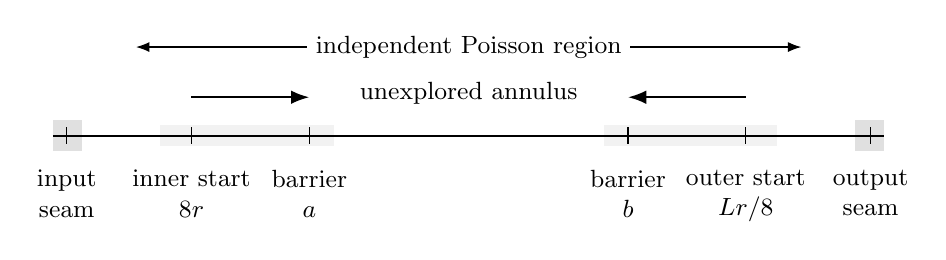
\begin{tikzpicture}[x=0.88cm,y=0.75cm,>=Latex,font=\small]
  \fill[black!12] (0,-0.26) rectangle (0.42,0.26);
  \fill[black!12] (11.58,-0.26) rectangle (12,0.26);
  \fill[black!5] (1.55,-0.18) rectangle (4.05,0.18);
  \fill[black!5] (7.95,-0.18) rectangle (10.45,0.18);
  \draw[thick] (0,0)--(12,0);
  \foreach \x in {0.2,2,3.7,8.3,10,11.8}
    \draw (\x,-0.14)--(\x,0.14);
  \node[align=center,below] at (0.2,-0.42) {input\\seam};
  \node[align=center,below] at (2,-0.42) {inner start\\$8r$};
  \node[align=center,below] at (3.7,-0.42) {barrier\\$a$};
  \node[align=center,below] at (8.3,-0.42) {barrier\\$b$};
  \node[align=center,below] at (10,-0.42) {outer start\\$Lr/8$};
  \node[align=center,below] at (11.8,-0.42) {output\\seam};
  \draw[->,thick] (2,0.65)--(3.7,0.65);
  \draw[->,thick] (10,0.65)--(8.3,0.65);
  \node[align=center] at (6,0.72) {unexplored annulus};
  \draw[<->] (1.2,1.5)--(10.8,1.5);
  \node[fill=white,inner sep=3pt] at (6,1.5) {independent Poisson region};
\end{tikzpicture}
\caption{The radial order of two end experiments with separated barriers,
on a schematic logarithmic scale.  Explorations start inside the transfer
block, independently of its two seams.  Each shaded end support extends
a little beyond its last barrier; the gap between those supports permits
their independent integration.  The original seam screens remain
imposed throughout.}
\label{tr:figure}
\end{figure}

The following elementary observation is the uniformity mechanism used
below.  Its purpose is to avoid any assertion of a uniform scaling
limit conditional on an atypical explored shape.

\begin{lemma}[Domination before conditioning on end shapes]
\label{tr:domination}
Suppose a contribution to $M_{r,Lr}v$ is expressed, after exploring from
the auxiliary starting cycles, as an integral of an inner scalar
coefficient, a bounded middle test, and an outer signed state measure.
If the middle test is replaced with absolute error $F\ge0$, where $F$
depends only on the independent region just described, then the error
in output norm is at most
\begin{equation}
              C\|v\|_r\,\E_{\mathrm{core}}F+o(1)\|v\|_r.
\label{tr:domination-bound}
\end{equation}
The same bound applies to discarding an event there, by taking $F$ to
be its indicator.  The expectation is under the unweighted full-plane
comparison law; the bound is uniform over successful output seams.
\end{lemma}

\begin{proof}
For a fixed realization, pushing $v_{\Sigma_r}$ to any intermediate
state set contracts total variation.  When that set has two states, its
zero-mass image has the form $\alpha(\delta_B-\delta_W)$, with
$|\alpha|\le\|v\|_r$.  Pushing the two-state difference through the other
end gives a signed measure $q$ with $\|q\|_{\TV}\le2$.  Hence the
pointwise norm of the replacement error is bounded by
$2\|v\|_rF$.  The same argument, summing absolute masses before a
two-state reduction, handles discarded events.  No regularity of the
dependence of $\alpha$ or $q$ on the seam data is needed.

On the auxiliary localization successes, $F$ is a function of marked
Poisson variables independent of both original seams and has the stated
full-plane comparison law.  Integrate the pointwise bound conditional
on the output seam.  Auxiliary failures contribute the final $o(1)$
term, also uniformly, because their supports are off the original seams.
The seam success indicators themselves are not deleted.
\end{proof}

\subsection{Exploration up to the first four-tip frontier}

First push the input message from its original seam to the inner
auxiliary starting cycle, using the marked variables in the intervening
attachment region.  The subsequent exploration uses the colored
starting cycle and the variables towards its barrier; it never consults
an attached cap state.  Dependence on the input message stays in the
pushed signed coefficients.  At the outer end the corresponding
attachment operation pushes states from its auxiliary cycle towards
the original output seam.

At the inner auxiliary cycle, reveal its colors and trace every switch
into the annulus.  A wall is followed until it pairs with another traced
wall or until its next color query would read a vertex on the current
barrier.  In the second case, stop before that query.  The stopped wall
ends at a switch edge whose next triangle has its opposite vertex on
the barrier.  No barrier colors have been read.  The analogous outer
experiment is directed inwards.  Increasing the inner barrier radius
by a factor two, or decreasing the outer barrier radius by a factor
two, continues the same wall system.  Tracing all walls in a previously
colored sample shows that the outcome does not depend on their tracing
order.

We call the unpaired stopped wall ends the \emph{surviving tips}.
Their number is even and decreases as the barrier is advanced.  The
first barrier with at most four surviving tips will be the end's
reduction barrier.  A reduction to zero or two tips kills every
zero-mass message.  A reduction to exactly four leaves precisely two
cap states.  We next verify both this assertion and the geometric
properties needed for the annular transmission limit.

\begin{lemma}[Frontier and arm counts]
\label{tr:frontier}
For either end experiment, outside an event whose probability tends to
zero as the permitted separation of tips tends to zero, mesh first,
the tips at each of finitely many fixed-scale barriers have distinct
limiting positions.  The boundary facing the unqueried barrier is a
simple site cycle whose switches are exactly these tips.  In particular:
\begin{enumerate}
\item If there are zero or two tips, the induced map on zero-mass
connection-state measures is zero.
\item If there are at least six tips, six disjoint bulk arms cross the
region from the starting cycle to the barrier, after fixed-factor
crops at the two ends.
\end{enumerate}
All probabilistic assertions are made under the unweighted exploration
law, before conditioning on a particular history.
\end{lemma}

\begin{proof}
First consider two tips approaching the same point of the barrier.
Use a graph disk patch with its base on the barrier and a half-annulus
on the exploration side.  Extend each stopped wall through its last
triangle to the base, only for this geometric argument; no barrier
color is queried.  The two wall fingers give two proper traversals of
the half-annulus, with fixed margins at its two semicircular ends.
Following the sites on their banks gives three disjoint free arms in
the sectors on the two exterior sides and between the fingers.  These
sites are on the exploration side, not on the barrier.  Short spokes
through successive wall triangles keep each bank in its sector.  The
base through the tips prevents an exterior bank from escaping around
a finger's end.  Cropping the last mesh steps gives the same count
when two stopping triangles share a barrier vertex.

This is the free-bank-shadow count for two traversals in the boundary
argument of \cite[Section~3]{V}.  The local boundary three-arm exponent
is strictly greater than one.  Covering the barrier by $O(s^{-1})$
patches of radius $s$ therefore excludes colliding tips as $s\downarrow0$,
mesh first.  The BK inequality applied to the free shadows also makes
the number of fixed-scale traversals tight.

For the frontier assertion, fill the starting side of the starting
cycle with a disk, using the sphere for the outside experiment.
Attach the queried triangles along the explored bands and add all
edges between revealed vertices.  The resulting graph is
two-connected: attaching a triangle along an existing edge preserves
two-connectivity, as does adding an edge between existing vertices.
Thus the boundary of its face containing the unqueried barrier is a
simple cycle.  The barrier and its paths towards the unexplored middle
remain in that face.  In particular each stopping triangle is incident
with this same face on its unread side.

There is a useful invariant: every revealed vertex has a revealed path
of its own color to the starting cycle.  It holds initially, and a newly
queried triangle vertex has the color of one endpoint of the incoming
heterochromatic edge, extending such a path.  Thus an added
heterochromatic edge between revealed vertices cannot belong to an
unstarted wall.  Such a wall would either close in the annulus or return
to the barrier without visiting the starting cycle; in either case it
would separate one bank from that cycle, contradicting its revealed
same-color path.  Every heterochromatic revealed-vertex edge therefore
belongs to the traced wall system.

To identify the colors along the frontier, extend the stopped walls
to the barrier as above.  These proper arcs, together with the walls
that paired back to the starting cycle, divide the explored collar
into regions with their consistent bank colors.  Every revealed vertex
is either a starting-cycle vertex or was queried in a wall triangle.
Its color agrees with the relevant bank.  An added edge cannot cross
one of these wall arcs, and the preceding invariant excludes any
untraced switch there.  Previously crossed switch edges have triangles on
both sides in the revealed bands.  The only switches exposed to the
remaining face are consequently the surviving stopping edges.

With zero or two switches there is just one noncrossing cap pairing.
Every input state gives that same pairing, so a zero-mass difference
vanishes.  With six or more surviving wall fingers, their bank shadows
give six disjoint site arms in successive sectors between the starting
cycle and the barrier.  Fixed-factor crops remove the two ends, where
different shadows could otherwise meet.  The arbitrary-color six-arm
bound is applicable, so no particular numbering or color order of the
six arms is required.
\end{proof}

The next lemma verifies the non-Jordan boundary issue rather than
presuming that scalar Cardy convergence applies to a random annulus.

\begin{lemma}[Admissibility of four-tip frontiers]
\label{tr:admissible}
At a fixed barrier, restrict the unweighted exploration law to the event
of exactly four surviving tips.  Along subsequences with good geometry
as in \cite[Section~2]{V}, the four monochromatic frontier arcs are tight
in curve order.  In every coupled subsequential limit, after constant
pauses are erased, each arc is simple and meets the stopping circle
only at its two prescribed endpoints.  The four endpoints are distinct.

For two such experiments ending at well-separated barriers, their
residual annulus satisfies the admissibility conditions of
Proposition~\ref{an:limit}.  If $t_r$ is the discrete
through-transmission probability conditional on the complete geometry
and the two end histories, and $T_r$
is the continuum transmission function evaluated on its actual
conformal data, then, for fixed $L$ and the fixed finite list of barriers,
\begin{equation}
       \E_{\mathrm{core}}\!\left[
          \boldsymbol 1_{\{\text{four tips at both ends}\}}
                              |t_r-T_r|\right]=o(1).
\label{tr:mean-limit}
\end{equation}
The expectation concerns unweighted histories, not a uniform conditional
estimate for all possible histories.
\end{lemma}

\begin{proof}
The BK and successive-excursion argument gives tightness of the four
frontier arcs.  Indeed repeated annular traversals provide disjoint
free arms; all sites used, including those on the auxiliary starting
cycle, have their original fair colors.  This is applied first at
fixed radii and then at successively smaller excursion scales.
The contact arguments below are the face-boundary arguments in
\cite[Section~3]{V}; we give the details relevant to the present
frontier.

Every frontier vertex off the starting cycle belongs to a revealed
wall band.  On its revealed side it has an opposite-colored neighbor
with a bank path back to the starting cycle.  Consequently a visit of
a frontier arc to the stopping circle other than at its designated
endpoint, with a positive excursion on both sides of the visit, gives
three free arms in a half-patch: two along the arc and one along the
opposite bank.  The same argument excludes an intermediate return to
an endpoint.  The boundary three-arm exponent and a covering of the
circle exclude all such visits.  A nonconstant interval contained in
the circle is excluded by the one-arm bound at a countable dense set
of circle points.  Constant pauses can be removed from the
parametrization.  Distinctness of the four tips follows from
Lemma~\ref{tr:frontier}.

Consider next a self-return of one monochromatic frontier arc at a
point away from the starting and stopping circles.  Separate the two
visits by a fixed positive excursion scale.  In a smaller annulus
around the proposed contact, the arc supplies four proper traversals.
Its opposite bank paths lie on the revealed side of the frontier
cycle.  They may all be joined through the starting cycle when making
the planar separation argument.  This joining set need not be
monochromatic at the starting cycle: the working annulus misses that
cycle, and within the working annulus every part of the joining set
is genuinely of the opposite color.

At least two complementary sectors have a frontier traversal on their
boundary whose revealed side faces the sector.  Each such sector
contains an opposite-colored longitudinal crossing.  To verify this assertion,
choose transverse cuts at intermediate scales with margins, leaving
both ends of that frontier traversal beyond the cuts.  If the joined
neighbor set did not cross the sector longitudinally, planar duality
would provide a transverse crosscut avoiding it.  Start this crosscut
from that frontier traversal and stop at its first subsequent hit of the
frontier cycle.  In the disk on the revealed side, the two traversal ends
and the two crosscut ends alternate along the frontier.  The crosscut
therefore separates their neighbor spokes, contradicting the joined
neighbor set, which lies on the revealed side and avoids the
crosscut.

The argument remains valid when the traversals backtrack.  Choose the
transverse cuts along intermediate graph cycles, or apply Hex duality
with such a cycle temporarily wired in the sector.  Two disjoint cuts
bound a quadrilateral whose side arcs belong to the chosen traversals
and whose interior avoids those whole proper traversals, not merely
the selected side subarcs.  Thus the crosscut's first subsequent
frontier hit lies outside the whole traversal from which it started,
so the alternating boundary order used above persists under
backtracking.  The crosscut is in the quadrilateral's interior, whereas the end spokes are beyond
the cuts.  They thus avoid the crosscut even if other portions of the
frontier enter the sector.  Cropping the margins leaves two disjoint
opposite-colored arms in different sectors, in addition to the four
arms along the monochromatic arc.  This gives six disjoint bulk arms.
The bulk exponent strictly greater than two excludes these contacts
by a covering argument.  At a self-contact on the starting circle,
the four arc traversals alone suffice: the arbitrary-color four-arm
exponent is strictly greater than one, and the possible contact
locations lie on a fixed circle.

All these exclusions are made for distinct visits with fixed positive
excursion scales before those scales decrease.  Countably many scales
and finite ball coverings make the assertions simultaneous.  They
bound joint probabilities with the four-tip event; no division by the
probability of a rare history is involved.

We now identify the remaining domain; see
Figure~\ref{fig:frontier-lobes}.  Cut along the barrier, using the
four short incidences from the tip edges through their terminal
triangles.  Between consecutive tips, the frontier arc and its
corresponding barrier interval bound a lobe polygon.  The four lobes
are attached over open intervals to the untouched region on the middle
side of the barrier.  Each lobe converges in order to a Jordan lobe,
because its frontier arc is simple and meets the barrier only at its
endpoints.  Different lobe boundaries may touch in physical projection;
their interiors remain disjoint, and their distinct accesses are
retained.  With two well-separated barriers there is a fixed open
annular region between the ends.

We verify that adjoining the lobes still gives an annulus, even when
their boundaries touch.  On either side of this open annular region,
start with the closed disk bounded by the corresponding stopping circle,
using the sphere for the outer side.  The complementary set on that
side is obtained by removing the lobe interiors and their open
attachment intervals.  Each lobe's free frontier arc remains in this
complement: it cannot enter another lobe's interior, since their Jordan
interiors are disjoint, and it meets the stopping circle only at its
own endpoints, never on another open attachment.  Connect a point of
the remaining closed set to the preserved starting-side region by a
path in the closed disk, with its interior off the stopping circle.
Whenever the path enters a lobe, replace the portion from its first
entry to its last exit by the intervening subarc of that lobe's free
frontier.  The entry and exit lie on this free arc.  The replacement
avoids every lobe interior and every open attachment, so it cannot
undo previous replacements.  There are only four lobes; after finitely
many replacements the path is wholly in the complementary set.
Thus each side has a connected complement.  The two such nondegenerate
continua are separated by the open annular region and exhaust the
complement of the residual domain.  The domain is therefore doubly
connected, with its two boundary components physically apart.

Lemma~\ref{an:back-lobes} now gives uniform convergence
of the closed-annulus parametrizations with their prime-end order.
The boundary traversal consists of finitely many individually simple
arcs.  These are exactly the hypotheses required by
Proposition~\ref{an:limit}.

Finally extract, from any sequence of scales, a further sequence on
which the localized full-plane geometries are good in the sense of
\cite[Section~2]{V}.  Conditional on those geometries, couple convergent
subsequences of the frontier histories just described.  All unqueried
colors in the residual face remain independent and fair.  Apply
Proposition~\ref{an:limit} path by path to the converging graph annuli.
The continuum function on the actual approximating conformal data
also converges, by its continuity.  Bounded convergence proves
\eqref{tr:mean-limit} along the further sequence and hence along the
original sequence.  Unused colors on the removed sides of the
frontiers may be revealed or integrated in their own end variables;
they do not affect this argument.
\end{proof}

\begin{figure}[tb]
\centering
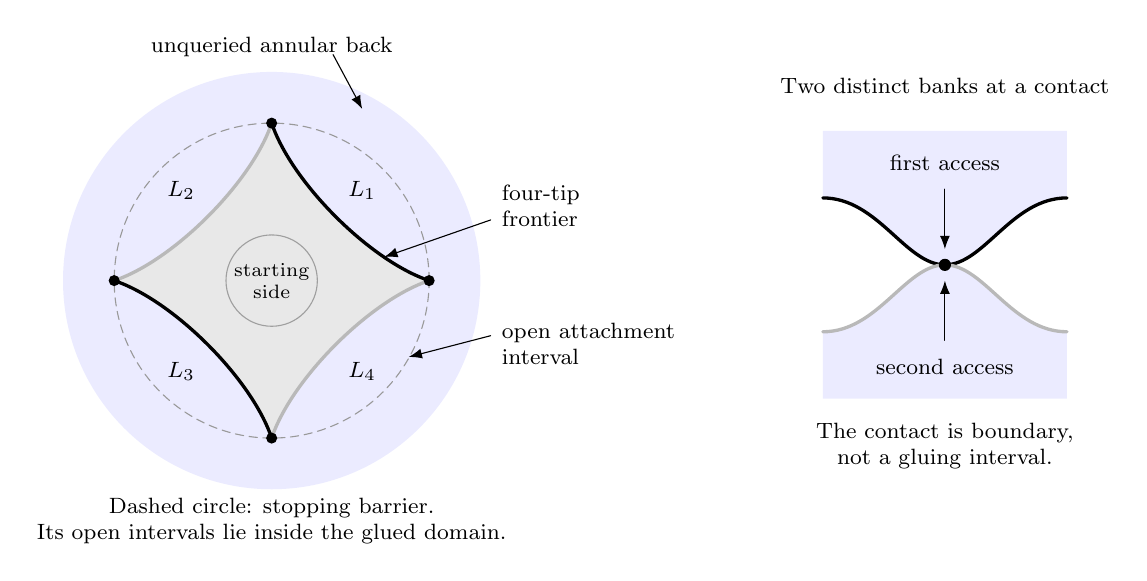
\begin{tikzpicture}[font=\footnotesize,>=Latex,line cap=round,
  bank/.style={very thick},
  barrier/.style={densely dashed,gray!80},
  fluid/.style={fill=blue!8}]
  \begin{scope}[xshift=0.3cm]
    \fill[blue!8] (0,0) circle (2.65);
    \fill[black!9]
      (2,0) .. controls (1.25,.25) and (.25,1.25) .. (0,2)
      .. controls (-.25,1.25) and (-1.25,.25) .. (-2,0)
      .. controls (-1.25,-.25) and (-.25,-1.25) .. (0,-2)
      .. controls (.25,-1.25) and (1.25,-.25) .. cycle;
    \draw[barrier] (0,0) circle (2);
    \draw[bank]
      (2,0) .. controls (1.25,.25) and (.25,1.25) .. (0,2);
    \draw[bank,gray!55]
      (0,2) .. controls (-.25,1.25) and (-1.25,.25) .. (-2,0);
    \draw[bank]
      (-2,0) .. controls (-1.25,-.25) and (-.25,-1.25) .. (0,-2);
    \draw[bank,gray!55]
      (0,-2) .. controls (.25,-1.25) and (1.25,-.25) .. (2,0);
    \foreach \p in {(2,0),(0,2),(-2,0),(0,-2)}
      \fill \p circle (2pt);
    \draw[gray!75] (0,0) circle (.58);
    \node[align=center,font=\scriptsize] at (0,0) {starting\\side};
    \node at (1.15,1.15) {$L_1$};
    \node at (-1.15,1.15) {$L_2$};
    \node at (-1.15,-1.15) {$L_3$};
    \node at (1.15,-1.15) {$L_4$};
    \node[align=center] at (0,2.97) {unqueried annular back};
    \draw[->,thin] (.78,2.87)--(1.15,2.18);
    \node[align=left,anchor=west] at (2.8,.95)
      {four-tip\\frontier};
    \draw[->,thin] (2.78,.77)--(1.43,.30);
    \node[align=left,anchor=west] at (2.8,-.80)
      {open attachment\\interval};
    \draw[->,thin] (2.78,-.70)--(1.74,-.97);
    \node[align=center] at (0,-3.05)
      {Dashed circle: stopping barrier.\\
       Its open intervals lie inside the glued domain.};
  \end{scope}

  \begin{scope}[xshift=8.85cm,yshift=.20cm]
    \node[align=center] at (0,2.28) {Two distinct banks at a contact};
    \fill[blue!8]
      (-1.55,1.70)--(1.55,1.70)--(1.55,.85)
      .. controls (.85,.85) and (.50,0) .. (0,0)
      .. controls (-.50,0) and (-.85,.85) .. (-1.55,.85)--cycle;
    \fill[blue!8]
      (-1.55,-1.70)--(1.55,-1.70)--(1.55,-.85)
      .. controls (.85,-.85) and (.50,0) .. (0,0)
      .. controls (-.50,0) and (-.85,-.85) .. (-1.55,-.85)--cycle;
    \draw[bank]
      (-1.55,.85) .. controls (-.85,.85) and (-.50,0) .. (0,0)
      .. controls (.50,0) and (.85,.85) .. (1.55,.85);
    \draw[bank,gray!55]
      (-1.55,-.85) .. controls (-.85,-.85) and (-.50,0) .. (0,0)
      .. controls (.50,0) and (.85,-.85) .. (1.55,-.85);
    \fill (0,0) circle (2.2pt);
    \node at (0,1.30) {first access};
    \node at (0,-1.30) {second access};
    \draw[->,thin] (0,.96)--(0,.20);
    \draw[->,thin] (0,-.96)--(0,-.20);
    \node[align=center] at (0,-2.30)
      {The contact is boundary,\\not a gluing interval.};
  \end{scope}
\end{tikzpicture}
\caption{The decomposition at an inner four-tip frontier. The four
monochromatic frontier arcs, drawn alternately black and gray, bound
Jordan lobes $L_1,\ldots,L_4$ with the stopping barrier. Each lobe is
attached to the untouched annular back along an open barrier interval;
the common shading denotes the resulting unqueried domain. The starting
side remains in the complement. At the other end the construction is
reversed. The inset records two accesses at a possible contact between
different banks: the contact is not added to the fluid and does not join
the accesses. All curves are schematic. Actual banks may be rough and
may touch each other, although each individual frontier arc is simple.}
\label{fig:frontier-lobes}
\end{figure}


The probabilistic conclusions of the last two lemmas all concern the
independent region.  Lemma~\ref{tr:domination} therefore makes their
discarded probabilities and the error in \eqref{tr:mean-limit} uniform
for the operator norm, even when a message depends arbitrarily on the
seam and on its attachment information.  This is the reason the
explorations start at auxiliary cycles rather than at the original
seams.

\subsection{The first-reduction decomposition}

Index the inner barriers by radii
\[
             a_j=8\cdot2^j r,
\qquad j=1,2,\ldots,
\]
and the outer barriers by
\[
             b_k=2^{-k}Lr/8,
\qquad k=1,2,\ldots.
\]
Each list is finite, ending before the opposite starting region.  Fix
a large integer $d$ so that
\begin{equation}
                  j+k\le n-d
\label{tr:used-pairs}
\end{equation}
ensures disjoint buffered end supports and sufficient separation for
Proposition~\ref{sh:separated-ends}.  A \emph{used pair} is a pair
satisfying \eqref{tr:used-pairs} at which the two experiments first
reduce to exactly four tips.  A first reduction to fewer than four
contributes zero by Lemma~\ref{tr:frontier}.

Choose $\tau>0$ smaller than the excess of the mesh-first six-arm
exponent over two.  Let $\rho_j^{\rm in}$ and $\rho_k^{\rm out}$ be the
subprobability laws of the corresponding first four-tip histories,
including local screens and the variables attaching each history to its
original seam.  The inner law integrates the input seam.  All outer
laws and outer integrals below are conditional on the fixed output seam
$\Sigma_{Lr}$; in particular they define fields over that seam, not
averages of it.  The dependence on seam variables in the
attachments will be kept in the scalar and signed measure factors
below, rather than in any assertion about typical shapes.  We first
bound the masses of these unweighted history laws; pointwise bounded
message factors will then preserve the bounds up to constants.

\begin{lemma}[First-reduction tails]
\label{tr:tails}
For fixed $L$, the end-history subprobability masses satisfy, in the
mesh-first limit,
\begin{equation}
 \|\rho_j^{\rm in}\|_{\TV}
 \operatorname*{ess\,sup}_{\Sigma_{Lr}}
         \|\rho_k^{\rm out}(\cdot\mid\Sigma_{Lr})\|_{\TV}
      \le C 2^{-(2+\tau)j}2^{-(2+\tau)k}+o(1)
\label{tr:history-weight}
\end{equation}
for each used pair $(j,k)$.  Consequently, after inserting arbitrary
middle tests of modulus at most one, the same bound up to a constant holds
for the corresponding operator contribution on inputs of norm at most
one.  The part of the transfer not represented
by used pairs has norm at most
\begin{equation}
             C(n+1)^2L^{-2-\tau}+o(1).
\label{tr:unused}
\end{equation}
Both estimates are uniform for input messages of norm at most one and
for successful output seams.
\end{lemma}

\begin{proof}
Before the first reduction at level $j$, there are at least six tips
at the preceding level.  Lemma~\ref{tr:frontier} then requires six arms
from the starting region to that level.  The mesh-first six-arm bound
gives $C2^{-(2+\tau)j}$, with a changed constant for the first few
levels.  The same statement holds at the outer end, uniformly in its
original seam: the necessary six-arm event is read in the independent
region, while attachment variables and success indicators have total
conditional mass at most one.  Multiplying the two separate mass
bounds proves \eqref{tr:history-weight}.  For used pairs the physical
end experiments also have disjoint buffered supports, so their joint
law is the product used in the operator contribution.  Arbitrary input
weights are bounded
pointwise by their total variation, as in
Lemma~\ref{tr:domination}; the number of switches on the input seam
does not enter the estimate.

To bound the remainder, run the inner exploration to its longest
allowed level.  If it never reduces, it has paid a six-arm probability
over $n-O(1)$ dyadic levels.  Otherwise let $j$ be its first reduction
level.  If the reduction has fewer than four tips, its contribution
is zero.  In the remaining case run the outer experiment as far as
\eqref{tr:used-pairs} allows, possibly through no additional level.
If it does not reduce in time, the two experiments together have
paid six-arm probabilities over at least $n-O(1)$ levels.  Their
buffered supports remain disjoint.  Summing the resulting bounds over
the at most $O((n+1)^2)$ possible terminal levels proves
\eqref{tr:unused}.  The finitely many auxiliary localization failures
and near-coincidences of tips cost $o(1)$ for fixed $L$, uniformly by
Lemma~\ref{tr:domination}.
\end{proof}

At a four-tip inner frontier let $B$ and $W$ denote respectively the
black-join and white-join cap states.  The pushed input message is
\begin{equation}
                 \alpha_j(v;H_i)(\delta_B-\delta_W),
                 \qquad |\alpha_j(v;H_i)|\le\|v\|_r,
\label{tr:inner-coefficient}
\end{equation}
where $H_i$ includes the inner history and its attachment to the input
seam.  The coefficient is linear in $v$.  Similarly, pushing
$\delta_B-\delta_W$ from an outer four-tip frontier to the output seam
gives a signed measure $q_k(H_o)$ satisfying
\begin{equation}
                         \|q_k(H_o)\|_{\TV}\le2.
\label{tr:outer-coefficient}
\end{equation}
Lemma~\ref{an:caps} says that the residual annulus sends the first
cap difference to the second multiplied by its through-transmission
probability.  Thus the used-pair contribution has the form
\begin{equation}
 \int \alpha_j(v;H_i)\,
       \E_{\rm mid}\!\left[
          \boldsymbol1_{G_{\rm aux}}t_r\mid H_i,H_o\right]
       q_k(H_o)\,d\rho_j^{\rm in}(H_i)d\rho_k^{\rm out}(H_o),
\label{tr:integral}
\end{equation}
where $G_{\rm aux}$ denotes the additional middle screens and
$\E_{\rm mid}$ integrates the middle Poisson geometry conditional on
the two end histories.  The probability $t_r$ already integrates the
fresh colors in the remaining face, conditional on all geometry.
The end laws are a product because their buffered supports are
disjoint.  The conditional factor in square brackets still couples
the ends, and must not yet be factored.

On the auxiliary localization successes, the residual frontiers and
both $t_r$ and $T_r$ depend only on the auxiliary-cycle explorations and
the intervening independent geometry.  Attachments to the original
seams enter only the signed coefficients.  The error $|t_r-T_r|$ thus
has exactly the independent-region measurability required by
Lemma~\ref{tr:domination}.

By Lemmas~\ref{tr:admissible} and~\ref{tr:domination}, replace $t_r$ by
$T_r$ in \eqref{tr:integral} with $o(1)\|v\|_r$ error in output norm.
For fixed $n$, this error may be summed over all used pairs.  The
frontiers themselves are still the actual graph cycles.  Their
single-end conformal maps and capacities can therefore be used
directly in Proposition~\ref{sh:separated-ends}, without asserting
smoothness at contacts of a limiting boundary.

\subsection{Rank-one factorization and signed cancellation}

We now complete Proposition~\ref{tr:block}.  An inner frontier at
level $j$ surrounds the center, stays inside radius comparable to
$a_j$, and reaches that radius at its tips.  Its logarithmic capacity
$l_i$ is therefore comparable to $a_j$.  An outer frontier at level
$k$ surrounds a disk of radius comparable to $b_k$ and has a point
at distance comparable to $b_k$; its conformal radius $l_o$ is
comparable to $b_k$.  Write $y^0$ and $x^0$ for their single-end
switch angles.  By \eqref{sh:rank-one},
\begin{equation}
 T_r(H_i,H_o)=K\,U(H_i)V(H_o)
                       +O\big((a_j/b_k)^{\lambda+\sigma_1}\big),
\label{tr:separated-formula}
\end{equation}
where
\[
 U(H_i)=l_i^\lambda J(y^0)^{1/3},
 \qquad
 V(H_o)=l_o^{-\lambda}J(x^0)^{1/3}.
\]
These factors depend on their own end histories only, and
\begin{equation}
             |U(H_i)V(H_o)|
                  \le C L^{-\lambda}2^{\lambda(j+k)}.
\label{tr:factor-size}
\end{equation}

For the separated leading term, delete the extra middle screens.
This changes the integral by $o(1)\|v\|_r$ for fixed $L$: the screens
use independent interior variables and fail with probability $o(1)$,
while all weights at these fixed scales are bounded.  Keep the original
seam screens and the local end screens.  The remaining end experiments
now use disjoint Poisson supports for every used pair.  Define the
scalar functionals and output messages
\[
 u_j(v)=\int \alpha_j(v;H_i)U(H_i)\,d\rho_j^{\rm in}(H_i),
 \qquad
 v_k=\int V(H_o)q_k(H_o)\,d\rho_k^{\rm out}(H_o).
\]
The leading contribution of that pair is exactly $K u_j(v)v_k$.
The same definitions make sense separately for every level in each
finite list, whether or not a pair of levels has disjoint supports.
For such additional pairs we use the product of the two separate
integrals, not a claim about simultaneous experiments.

Set
\begin{equation}
       M_1v=K\left(\sum_j u_j(v)\right)\left(\sum_k v_k\right).
\label{tr:rank-one-definition}
\end{equation}
This operator has rank at most one.  By the separate six-arm bounds
and \eqref{tr:factor-size}, its norm is at most
\begin{equation}
 C L^{-\lambda}
       \sum_{j,k}2^{-(2+\tau-\lambda)(j+k)}
                   \le C L^{-\lambda}.
\label{tr:rank-one-size}
\end{equation}
The extra product terms introduced by allowing $j+k>n-d$ have norm
at most
\begin{equation}
 C L^{-\lambda}
      \sum_{j+k>n-d}2^{-(2+\tau-\lambda)(j+k)}
                   \le C(n+1)^2L^{-2-\tau}.
\label{tr:artificial-pairs}
\end{equation}
This numerical estimate requires no independence for overlapping
actual experiments.

Decrease $\sigma_1$ if necessary so that
$\lambda+\sigma_1<2+\tau$.  The errors in
\eqref{tr:separated-formula}, summed using
Lemma~\ref{tr:tails}, have norm at most
\begin{equation}
 C L^{-\lambda-\sigma_1}
      \sum_{j+k\le n-d}
             2^{-(2+\tau-\lambda-\sigma_1)(j+k)}+o(1)
       \le C L^{-\lambda-\sigma_1}+o(1).
\label{tr:rank-error-sum}
\end{equation}
Together with \eqref{tr:unused} and
\eqref{tr:artificial-pairs}, this proves the first two estimates of
Proposition~\ref{tr:block}, with a smaller positive exponent saving,
in the mesh-first limit.  All errors are measured in output total
variation, not merely after testing a fixed continuum event.

It remains to prove the stronger estimate for an even isotropic input
$v$.  After the continuum replacement, delete the extra middle screens
as above.  Only $T_r$ then depends on both ends; all other factors
belong to their separate, independently integrated end laws.
Rotate all inner end data, including the seam and the revealed
history.  By equivariance of $v$, the coefficient
$\alpha_j(v;H_i)$ in \eqref{tr:inner-coefficient} is unchanged.  Reverse
all colors of the inner data instead.  The message is still unchanged
as a geometrically transformed signed measure, but the reference
vector $\delta_B-\delta_W$ changes sign.  Thus
\begin{equation}
 \alpha_j(v;\operatorname{rot}_\theta H_i)=\alpha_j(v;H_i),
 \qquad
 \alpha_j(v;\operatorname{flip} H_i)=-\alpha_j(v;H_i).
\label{tr:coefficient-symmetry}
\end{equation}
The inner end law is rotation and color-reversal invariant.  The outer
measure factor is unaffected by either transformation of the inner
data.  Labels for the four tips may be chosen independently of colors
using the auxiliary angular axis, and transported under rotations.
For each fixed outer history $H_o$, color reversal gives the identity
\begin{equation}
\begin{aligned}
 &\int \alpha_j(v;H_i)T_r(H_i,H_o)\,d\rho_j^{\rm in}(H_i)\\
 &\quad=\frac12\int \alpha_j(v;H_i)
    \big[T_r(H_i,H_o)-T_r(\operatorname{flip}H_i,H_o)\big]
                                   \,d\rho_j^{\rm in}(H_i).
\end{aligned}
\label{tr:flip-integral}
\end{equation}
Now average rotations of the inner data in the right side.  Since
$\alpha_j$ and the inner law are rotation invariant, its contribution
is one half of the integral against the rotation average of
$T^+-T^-$, with its appropriate inner prescriptions.  In particular
one must retain the sign; replacing this difference by an unsigned
four-arm event would lose the required exponent.

Equation~\eqref{sh:rotation-average} bounds the averaged difference
by $C(a_j/b_k)^{2+\sigma_2}$.  The local end experiments and screens
can be chosen rotation and color-reversal invariant.  Decrease
$\sigma_2$ so that $0<\sigma_2<\tau$.  The used-pair contributions
are bounded in total variation by
\begin{equation}
 C L^{-2-\sigma_2}
    \sum_{j+k\le n-d}2^{-(\tau-\sigma_2)(j+k)}+o(1)
                  \le C L^{-2-\sigma_2}+o(1).
\label{tr:signed-sum}
\end{equation}
Adding the unused contribution \eqref{tr:unused} proves the desired
power strictly greater than two.

Finally choose $\delta>0$ smaller than all the positive savings just
obtained, decreasing it to absorb the polynomial factors in $n$.
For each fixed sufficiently large $n$, choose $r_0(2^n)$ so that every
$o(1)$ term is smaller than the required fixed power of $L$.  This
proves \eqref{tr:block-size}--\eqref{tr:block-cancellation}.
Notice the order: the ratio is chosen first and the scale threshold
afterwards.  No rate of convergence in Cardy's formula, in the
good-sequence extraction, or near a nonsimple limiting bank is used.

\subsection{Iteration and failed screens}

The block estimates have two consequences.  The first uses the signed
symmetry estimate to control a Poisson insertion.  The second uses the
rank-one approximation to compare two responses at different distant
boundaries.

\begin{corollary}[Fair-insertion message]
\label{tr:insertion}
There are $0<\nu<1$ and $C<\infty$ such that the following holds.  Insert
a nucleus at the center of a cut, with an independent fair color.  At
a seam of radius $s$, take the difference of the inside state laws
``with this insertion'' minus ``without this insertion,'' conditional
on the seam and with its screen success imposed.  Its message
$I_s$ satisfies
\begin{equation}
                            \|I_s\|_s\le C s^{-2-\nu}
\label{tr:insertion-bound}
\end{equation}
for all sufficiently large $s$.  The estimate remains valid in the
presence of fixed data outside the screened collar that do not enter
its inside.  The seam tests and the selected cycle are those of the
base process, without the insertion.
\end{corollary}

\begin{proof}
Choose a ratio $L$ from Proposition~\ref{tr:block} so large that the
constant per block in \eqref{tr:block-cancellation} is absorbed by a
smaller power saving.  Choose $s_*>r_0(L)$ sufficiently large.  For
given $s$, use radii
\[
             r_j=L^j r_0,\qquad 0\le j\le N,
             \qquad r_N=s,\quad s_*\le r_0<Ls_*.
\]
All screens use the base process.  At a successful seam, the inserted
point cannot reach or alter its cycle, by localization.  The two
inside state laws consequently have the same state space and each
has mass one.  Their difference has zero mass, norm at most two,
and is even and isotropic.

If every seam is successful, iterating
\eqref{tr:block-cancellation} bounds the message by
$C(s/r_0)^{-2-\nu}$ for some $0<\nu<1$.  Since $r_0$ stays in a fixed
compact range of positive scales, this gives
\eqref{tr:insertion-bound} for that contribution.

For the remaining contribution, group configurations by the largest
failed radius $v=r_j<s$.  The exact partition, with the final success
kept in every term, is
\[
 \boldsymbol1_{G_{r_N}}
   =\prod_{i=0}^{N}\boldsymbol1_{G_{r_i}}
    +\sum_{j=0}^{N-1}\boldsymbol1_{G_{r_j}^c}
                      \prod_{i=j+1}^{N}\boldsymbol1_{G_{r_i}}.
\]
Form a fresh difference of inside state
laws at the next cut $Lv=r_{j+1}$, multiplying both laws by the same
base-process indicator $\boldsymbol1_{G_v^c}$.  Earlier screen
outcomes are left unrestricted.  This weighted difference still has
zero mass for each successful seam at $Lv$: for each common base
configuration the two state laws have equal total mass.  It is also
even and isotropic.  The collar at $v$ is disjoint from that at $Lv$,
so conditional on the latter seam its norm is at most
\begin{equation}
                2\Pp(G_v^c\mid\Sigma_{Lv})
                           \le C e^{-cv^2}.
\label{tr:reset}
\end{equation}
Success at $Lv$ ensures that both configurations use the same cut
there, independently of what happened at smaller radii.

Transfer this reset message through the successful cuts above $Lv$.
Those success restrictions ensure that $v$ is indeed the largest
failed radius; no restriction on earlier failures was needed.
The sum of these contributions is bounded by
\[
 C\sum_{v\in\{r_0,\ldots,r_{N-1}\}}
             e^{-cv^2}\left(\frac{s}{Lv}\right)^{-2-\nu}
       \le C s^{-2-\nu}.
\]
The final inequality follows by summing the exponentially decaying
weights times $v^{2+\nu}$ over the geometric sequence.  This proves
the claim.  Outside data beyond the final screened collar have no
effect on the inside law or on the argument, which proves the stated
stability.
\end{proof}

For a message space $\mathcal B_t$, the projective norm on its algebraic
tensor square is
\[
 \|z\|_\pi
   =\inf\left\{\sum_{i=1}^m\|u_i\|_t\|v_i\|_t:
          z=\sum_{i=1}^m u_i\otimes v_i,\quad m<\infty\right\}.
\]
We may complete in this norm.  Bounded linear functionals $\ell,\ell'$
on $\mathcal B_t$ satisfy
\[
         |(\ell\otimes\ell')(z)|
                \le\|\ell\|\,\|\ell'\|\,\|z\|_\pi.
\]
In particular, evaluating $u\otimes v-v\otimes u$ gives the determinant
$\ell(u)\ell'(v)-\ell(v)\ell'(u)$.

\begin{corollary}[Contraction of antisymmetric products]
\label{tr:wedge}
There are $\nu'>0$, $s_0<\infty$, and a fixed ratio $L>1$ such that,
for $r\ge s_0$ and $s/r=L^N$, the transfer
\[
          \mathcal M=M_{s/L,s}\cdots M_{r,Lr}
\]
with all intermediate seam successes imposed satisfies
\begin{equation}
 \|\mathcal M u\wedge\mathcal M v\|_\pi
       \le C(s/r)^{-2\lambda-\nu'}\|u\|_r\|v\|_r
\label{tr:wedge-bound}
\end{equation}
for any two zero-mass input messages $u,v\in\mathcal B_r$.  Here
$u\wedge v=u\otimes v-v\otimes u$ and $\|\cdot\|_\pi$ is the
projective tensor norm.  Fixed-factor unused intervals at the two
ends change only the constant.  No assertion of this contraction
through a failed intermediate cut is made.
\end{corollary}

\begin{proof}
For one block write $M=M_1+E$ as in
\eqref{tr:block-rank}.  Since $M_1$ has rank at most one,
$M_1\otimes M_1$ vanishes on antisymmetric tensors.  On that subspace,
\[
 \|M\otimes M\|
        \le 2\|M_1\|\,\|E\|+\|E\|^2
        \le C L^{-2\lambda-\delta}.
\]
Choose $L$ large enough to absorb $C$ into a smaller exponent saving
$\nu'>0$, simultaneously with its choice in
Corollary~\ref{tr:insertion}.  Iterating the estimate and using
$\|u\wedge v\|_\pi\le2\|u\|_r\|v\|_r$ gives
\eqref{tr:wedge-bound}.  The argument holds first for finite tensor
sums and then for their projective-norm completion.  Ordinary
Markov pushes contract total variation, so fixed-factor omitted end
intervals affect only the constant after rounding to the ratio-$L$
grid.
\end{proof}

\section{The intensity derivative and the pivotal amplitude}
\label{sec:amplitude}

The preceding section supplies two estimates with different roles.
Corollary~\ref{tr:insertion} makes the effect of a distant fair insertion
integrable, even after division by the central pivotal probability.
Corollary~\ref{tr:wedge} makes the normalized effect of a nearby insertion
almost independent of the size of the rectangle. Together they give a
summable error for the logarithmic derivative of $f$.
Throughout this section the Poisson intensity is one, unless otherwise
specified, and $\lambda=5/4$.

\subsection{Differentiating the intensity}

Let $X_R(\eta)$ be the indicator of a black left--right crossing of
$RQ_0$ for a colored point configuration $\eta$, with the closed-cell
convention of Theorem~\ref{thm:main}. If $0^{\rm b}$ and $0^{\rm w}$
denote an inserted black and white point at the origin, respectively, put
\[
 H_R(\eta)
 =X_R(\eta\cup\{0^{\rm b}\})-X_R(\eta\cup\{0^{\rm w}\}).
\]
Thus $H_R\in\{0,1\}$, and $f(R)=\E H_R(\eta)$ for the unit-intensity
fairly colored process. For $y\ne0$, write $y^{\rm f}$ for an independently
fairly colored inserted point and define
\begin{equation}\label{cl:kernel}
 K_R(y)=\E\bigl[H_R(\eta\cup\{y^{\rm f}\})-H_R(\eta)\bigr].
\end{equation}
The expectation includes the extra color. Values at $y=0$ and at null
nongeneric insertion locations are immaterial to the integrals below.
In particular, $K_R$ is an insertion difference of a \emph{color}-pivotal
probability, not a probability of Poisson pivotality.

\begin{lemma}[Intensity differentiation]\label{cl:derivative}
The function $f$ is continuously differentiable on $(0,\infty)$. For
every $R>0$, $K_R$ is absolutely integrable and
\begin{equation}\label{cl:derivative-eq}
 \frac R2 f'(R)=\int_{\R^2}K_R(y)\,dy.
\end{equation}
\end{lemma}

\begin{proof}
Let $\eta_t$ have intensity $t$ and fair colors. Euclidean scaling gives
\begin{equation}\label{cl:scaling-intensity}
 G_R(t):=\E H_R(\eta_t)=f(\sqrt t\,R).
\end{equation}
We justify differentiation of the full-plane expectation before using
this identity. All the estimates in this paragraph are uniform for
$t$ in a compact subinterval of $(0,\infty)$.

For $n\ge n_0(R)$, let $H_{R,n}$ be the same test computed from the
points in $B(0,2^n)$, together with the central insertion. A locality
screen in a collar well inside $B(0,2^n)$ determines every cell meeting
$RQ_0$, including its intersections with the boundary. Consequently
$H_{R,n}=H_R$ outside an event of probability at most
$C_R\exp(-c_R4^n)$. The same screen gives
$H_{R,n+1}=H_{R,n}$. Finite-volume Poisson differentiation follows by
differentiating the absolutely convergent Poisson series; see also
\cite[Theorem~19.1]{LP}. Equivalently,
for a bounded function $F$ of the process in a bounded set $D$,
\begin{equation}\label{cl:poisson-score}
 \frac{d}{dt}\E F(\eta_t\cap D)
 =\E\left[F(\eta_t\cap D)
       \left(\frac{N_t(D)}t-|D|\right)\right].
\end{equation}
Here $N_t(D)$ is the number of Poisson points in $D$.
Apply this to $F=H_{R,n+1}-H_{R,n}$ on $D=B(0,2^{n+1})$.
The score in parentheses has second moment $|D|/t$. Cauchy--Schwarz
therefore bounds the derivative by
$C_R2^n\exp(-c_R4^n)$. The differences of the expectations and of
their derivatives are uniformly summable. Hence $G_R$ is $C^1$ and
its derivative is the limit of the finite-volume derivatives.

The add-one version of finite-volume differentiation is
\[
 \frac{d}{dt}\E H_{R,n}(\eta_t)
 =\int_{B(0,2^n)}
  \E\bigl[H_{R,n}(\eta_t\cup\{y^{\rm f}\})
                     -H_{R,n}(\eta_t)\bigr]\,dy.
\]
For fixed $y$ the integrand converges to its full-plane counterpart.
For $|y|\ge C R+C$, a screen surrounding $RQ_0$ and the origin, at
distance comparable to $|y|$ and strictly short of $y$, prevents the
insertion from changing any cell used by the test. Its failure
probability is at most $C_R e^{-c_R|y|^2}$. The screen can be taken
inside $B(0,2^n)$ whenever $y\in B(0,2^n)$ and $n$ is sufficiently
large; thus this is also a dominating bound for the finite-volume
integrands. On a fixed bounded set the bound $2$ suffices.
Dominated convergence proves absolute integrability and identifies
$G_R'(1)$ with the integral in \eqref{cl:derivative-eq}.
Equation~\eqref{cl:scaling-intensity} proves the asserted derivative
formula and, locally at each $R$, the $C^1$ assertion for $f$.
\end{proof}

\subsection{An integrable tail after normalization}

The exponential localization in Lemma~\ref{cl:derivative} is a
finite-scale statement. We need a bound uniform as $R$ grows, with
the small factor $f(R)$ retained. This is where the signed insertion
estimate is essential.

\begin{lemma}[Normalized insertion tail]\label{cl:tail}
There are constants $\xi>0$, $m_0<\infty$, and $C<\infty$ such that
for $m_0\le m\le R/100$,
\begin{equation}\label{cl:tail-eq}
 \int_{|y|>m}|K_R(y)|\,dy
 \le C f(R)\bigl(m^{-\xi}+R^{-\xi}\bigr).
\end{equation}
\end{lemma}

\begin{proof}
Use the exponent $0<\nu<1$ of Corollary~\ref{tr:insertion} and
the one-arm exponent $\beta>0$ from the critical inputs. All screens
and arm probes below have fixed-factor buffers. Independent probes
mean probes determined by disjoint sets of Poisson coordinates,
not unrestricted Voronoi events in disjoint planar regions.

We first explain how arm requirements can be multiplied by a signed
message estimate. The integrand in \eqref{cl:kernel} is a mixed
difference: one difference changes the central color, and the other
inserts the point at $y$. If this mixed difference is nonzero, changing
the central color changes a crossing for at least one setting of the
insertion, and changing the insertion changes a crossing for at least
one setting of the central color. A screened probe separated from
both changes reads the same base colors in all four configurations.
Thus the necessary-arm implications for a local change apply to
these common colors; see \cite[Section~2, ``Necessary arms for a
local change'']{V}. They apply even when the two crossing changes
occur in different configurations.

The conditional version is equally important. Every formal noncrossing
pairing can be drawn as disjoint wall arcs in a topological disk.
Coloring its complementary regions alternately realizes the prescribed
boundary runs and the pairing. Thus two formal cap states give two
planar fillings agreeing on every exterior probe; the deterministic
necessary-arm argument does not require Poisson geometry inside the
replaced disk. Fix a successful
cut about $y$, its seam, and all exterior variables. The exterior
test is now a function of the inside connection state. If a
necessary central or enclosing four-arm event does not occur,
the central black-minus-white test is zero for every such state.
If a necessary side or corner arm event does not occur, each
crossing test with the central color fixed is constant across
inside states. These are
the same planar necessary-arm implications, applied to two
possible cap states on the cut. The insertion message has zero
mass, so it annihilates the latter constants. Its conditional
answer is consequently bounded by its total variation norm times
the necessary probe indicators. Those indicators are measurable
outside the cut. Disjoint buffered supports then allow their
probabilities to be multiplied.

We use screened arm probes with failures allowed, whose probabilities
are still bounded by a constant times their intended arm bounds;
see the convention in Section~\ref{sec:inputs} and
\cite[Section~2, ``Buffered localization'']{V}.
Indeed, group failures by the largest failed radius $v$ and retain
the arm test starting a fixed factor beyond $v$, independently of
the failure. For a four-arm probe starting at $r$, the relevant
estimate is
\[
 e^{-cv^2}A(C_0v,R)
 \le C A(r,R)(v/r)^g e^{-cv^2}
 \qquad(C_0v<R),
\]
where $g$ is the polynomial exponent in \eqref{in:power}.
For a side or corner probe the corresponding endpoint losses
are bounded by $C(v/d)^2$ or $C(v/u)^\beta$, respectively.
If a failed screen crosses the junction between side and corner
probes, the lost factors are therefore only polynomial. If the
retained test has no remaining radial range, the same comparison follows from the
polynomial lower bound, or directly from the displayed power
factor for a side or corner probe. Summing over geometric $v$
preserves the indicated arm cost as long as the retained probes
and the failure event have disjoint buffered supports. A failure
large enough to reach the central probe requires a separate
argument below: that probe is then dropped, not treated as
independent. An unweighted exponentially small error alone would
not suffice when $R$ is arbitrarily large.

\paragraph{Insertions near the center.}
Put $t=|y|$ and suppose $m<t\le R/100$. First fix a small
constant $c_1>0$, and then choose $a>0$ sufficiently small relative
to $c_1$. Choose a cut about $y$ of radius $a t$,
a central four-arm probe from $b_*$ to $a t$,
and a four-arm probe surrounding both insertions from $a^{-1}t$
to $aR$.
Short or overlapping endpoint ranges are omitted at constant cost.
The buffers of these three constructions can be chosen disjoint.
On cut success, Corollary~\ref{tr:insertion} gives a bound
$Ct^{-2-\nu}$ for the insertion message. The central color
difference requires the first four-arm probe; transmission of a
change from the region containing both insertions to the crossing
requires the second. Thus the success contribution is at most
$Ct^{-2-\nu}A(b_*,t)A(t,R)$.

For failures, let $v$ be the largest failed radius about $y$, with
the initial radius comparable to $t$. If $v<c_1t$, the
central probe and an enclosing
probe retain disjoint supports after the fixed buffer adjustments.
The preceding failed-screen estimate bounds their total
contribution by $Ce^{-ct^2}A(b_*,t)A(t,R)$.
If $v\ge c_1t$, drop the central probe. Retain instead a screened
four-arm probe centered at the origin, from radius $C_1(v+t)$
to $aR$, enclosing both modifications and with its support
separated from the failed screen. The same necessary-arm
implication supplies this probe. When its radial range is nonempty,
quasi-multiplicativity and \eqref{in:power} give
\[
 e^{-cv^2}A(C_1(v+t),aR)
 \le C A(b_*,R)(v+t)^g e^{-cv^2}.
\]
Since $t\le c_1^{-1}v$, summation over these geometric $v$ is
at most $C A(b_*,R)e^{-c't^2}$. If the retained radial range
is empty, then $R\le C(v+t)\le C'v$; the absolute failure
bound and $A(b_*,R)\ge cR^{-g}$ give the same conclusion.
Combining success and both failure cases proves
\begin{align}
 |K_R(y)|
 &\le Ct^{-2-\nu}A(b_*,t)A(t,R)
             +C A(b_*,R)e^{-ct^2}\notag\\
 &\le C f(R)t^{-2-\nu}.
 \label{cl:bulk-kernel}
\end{align}
In the last line we used quasi-multiplicativity and
\eqref{in:comparison}. In particular,
\begin{equation}\label{cl:bulk-integral}
 \int_{m<|y|\le R/100}|K_R(y)|\,dy
 \le C f(R)\int_m^\infty t^{-1-\nu}\,dt
 \le C f(R)m^{-\nu}.
\end{equation}

\paragraph{Insertions near a side or corner.}
Consider $R/100<|y|\le10R$, including points outside the rectangle.
Fix a sufficiently large constant $d_*$, and then a sufficiently
small constant $\rho>0$. If $\mathcal C_R$ is the set of the four
corners of $RQ_0$, set
\[
 d(y)=\min\{\rho R,\max\{d_*,\dist(y,\partial(RQ_0))\}\},
 \qquad
 u(y)=\min\{\rho R,\max\{d_*,\dist(y,\mathcal C_R)\}\}.
\]
We take $R$ large enough that $d_*<\rho R$. Always
$d_*\le d(y)\le u(y)\le\rho R$; write $d=d(y)$ and $u=u(y)$.
The constants in the estimates may depend on $d_*$ and $\rho$.
There is a central four-arm probe up to radius $cR$, where $c$
is fixed and much smaller than $1/100$, disjoint from the other
regions used below. Its cost is at most $CA(b_*,R)$.

At an interior point $y$, use the insertion estimate on a cut of
radius a small fixed fraction of $d$. At the bottom cutoff a
constant bound suffices, and can be bounded by $Cd^{-2-\nu}$
because $d_*$ is fixed. At an exterior point with distance above
the bottom cutoff, successful screening at this scale leaves the
quad unchanged. Only screen failures contribute there, with a bound
exponential in $d^2$, which is no larger than $Cd^{-2-\nu}$.

If $u/d$ is larger than a sufficiently large constant, the closest
part of the boundary is a straight side. A crossing change then
requires three alternating free arms in a half-plane probe centered
at the projection onto that side, from radius $Cd$ to radius $cu$.
Its cost is at most $C(d/u)^2$. If the projection is at a corner,
the two distances are comparable and this probe is unnecessary.
When $u$ is uncapped and is a sufficiently small fraction of $R$,
retain a one-arm probe centered at the nearest corner from radius
$Cu$ to radius $cR$. Its cost is at most $C(u/R)^\beta$.
For $u$ capped above, this factor is a fixed positive constant,
so the corresponding probe can be omitted. These are precisely
the local-change arm implications for the unwired, closed-cell
crossing convention. They also cover a modified cell meeting a
side or a corner.

The insertion cut, the side probe, the corner probe, and the
central probe can be given disjoint buffered supports. To arrange
this, first fix the central radius $cR$, then choose the distance
cap $\rho R$ much smaller. A corner probe is used only in a
corner neighborhood, far from the center. Fixed multiples are
lost between consecutive probes, which changes only constants.
To include failures, choose a sufficiently small fixed $c_2>0$.
For a largest failed radius $v<c_2R$ about $y$, the central
probe remains disjoint from the failed-screen support. Retain
the side and corner probes only beyond that support. If a
junction has been passed, the center of the affected side or
corner stage lies within $O(v)$ of $y$, so a fixed-factor
enlargement provides the required separation. Omitting an entire
side stage loses at most $C(1+v/d)^2$, and shifting or omitting
a corner stage loses at most $C(1+v/u)^\beta$. Since the first
possible failed radius is a fixed fraction of $d$,
\[
 \sum_{v\ge c_3d}e^{-cv^2}(1+v/d)^2(1+v/u)^\beta
 \le Cd^{-2-\nu}.
\]
The retained central probe supplies $A(b_*,R)$ throughout this
case. For $v\ge c_2R$, discard all arm probes and sum the
absolute failure probabilities, obtaining $Ce^{-c'R^2}$.
This is bounded by the right side of \eqref{cl:boundary-kernel}:
$A(b_*,R)\ge cR^{-g}$ and
$d_*\le d\le u\le\rho R$ make the reciprocal of that right
side at most a fixed power of $R$. This case includes every
failure whose support reaches the central probe, because
$|y|\ge R/100$ and the central probe radius was chosen much
smaller than $R/100$.
Thus no overlapping supports have been treated as independent.
The conditional total-variation argument on screen success,
together with these failure bounds, proves uniformly that
\begin{equation}\label{cl:boundary-kernel}
 |K_R(y)|\le C A(b_*,R)\,
     d^{-2-\nu}\left(\frac d u\right)^2
                    \left(\frac u R\right)^\beta.
\end{equation}

For completeness, a dyadic class with distances comparable to
$d,u$ has area at most $Cud$. Below the upper cap, it lies in
corner disks of radius $Cu$ and boundary strips of width $Cd$.
If $u$ is capped, the total strip length is $O(R)=O(u)$;
if both distances are capped, the ambient region has area
$O(R^2)=O(ud)$. These assertions apply equally outside the
rectangle. The bottom classes have the same bounds with $d_*$
in place of a smaller distance. Summing
\eqref{cl:boundary-kernel} first over dyadic $d\le u$ gives
\begin{align*}
 \sum_{d\le u} Cud\,d^{-2-\nu}(d/u)^2(u/R)^\beta
 &=\frac C u\left(\frac uR\right)^\beta
                           \sum_{d\le u}d^{1-\nu}\\
 &\le C u^{-\nu}(u/R)^\beta,
\end{align*}
where $\nu<1$ is used. The remaining dyadic sum is bounded by
\[
 C R^{-\beta}\sum_{d_*\le u\le\rho R}u^{\beta-\nu}
 \le C R^{-\xi_0}
 \qquad\text{for every }0<\xi_0<\min\{\beta,\nu\}.
\]
The strict inequality accommodates the logarithm when $\beta=\nu$.
Together with \eqref{in:comparison}, this proves
\begin{equation}\label{cl:boundary-integral}
 \int_{R/100<|y|\le10R}|K_R(y)|\,dy
 \le C f(R)R^{-\xi_0}.
\end{equation}

\paragraph{Far exterior insertions.}
For $|y|>10R$ an agreement screen between the test rectangle and
$y$ gives $|K_R(y)|\le Ce^{-c|y|^2}$. Its integral is at most
$Ce^{-cR^2}$. The polynomial lower bound for $f$ following from
\eqref{in:comparison} absorbs this into $Cf(R)R^{-\xi_0}$.
Combining this with \eqref{cl:bulk-integral} and
\eqref{cl:boundary-integral}, and decreasing the exponent, proves
\eqref{cl:tail-eq}.
\end{proof}

\subsection{Comparing the normalized derivatives}

The tail estimate permits us to discard insertions far from the
origin. For the remaining insertions we use the same interior
messages in two different rectangles. Rank-one approximation then
controls a determinant, so that no unknown leading factor needs
to be identified.

\begin{lemma}[Two-size determinant]\label{cl:determinant}
Let $\nu'>0$ be the exponent in Corollary~\ref{tr:wedge}.
There are constants $C,c>0$ such that, for sufficiently large $m$,
$100m\le R\le R'\le2R$, and almost every $0<|y|\le m$,
\begin{equation}\label{cl:determinant-eq}
 \bigl|K_R(y)f(R')-K_{R'}(y)f(R)\bigr|
 \le C(m/R)^{2\lambda+\nu'}+Ce^{-cm^2}.
\end{equation}
The constants are independent of the distance from $y$ to the origin.
\end{lemma}

\begin{proof}
Take concentric cuts about the origin, starting at radius $10m$
and ending at a radius comparable with a small fixed fraction of
$R$, with consecutive radii in ratio $L$. Round the final radius
down to the last such scale. Its ratio to $R$ is bounded below
by a positive constant depending only on the already fixed $L$.
All cut collars lie strictly inside both rectangles and outside
both inserted points. If necessary, enlarge the fixed lower
bound on $R/m$; the remaining bounded ratios follow by increasing
$C$, since all four scalar quantities in the determinant are bounded.

First restrict every test to success of every cut screen, with
the screens evaluated on the common base process. The probability
discarded is bounded by
\[
 C\sum_{j\ge0}\exp\bigl(-cm^2L^{2j}\bigr)
 \le Ce^{-c'm^2}.
\]
At the first cut let $a$ be the signed connection-state message
obtained by changing the central color. Let $b_y$ be the
difference of this message with and without the extra fair point
at $y$. Both have zero mass conditional on each seam, and
their total variation norms are bounded by $2$ and $4$,
respectively. They depend on neither $R$ nor $R'$: on screen
success their construction uses only the common interior
Poisson variables and the first seam. In particular this
description does not require disjoint neighborhoods of $0$ and $y$.

Let $T$ be the composed transfer through the intervening cuts.
The exterior crossing tests in $RQ_0$ and $R'Q_0$ define bounded
linear functionals $\ell_R$ and $\ell_{R'}$ at the final cut.
The four restricted expectations are
\[
 \ell_R(Ta),\quad \ell_{R'}(Ta),\quad
 \ell_R(Tb_y),\quad \ell_{R'}(Tb_y).
\]
Their determinant is the evaluation of $T^{\otimes2}$ on
$b_y\otimes a-a\otimes b_y$ by
$\ell_R\otimes\ell_{R'}$. Corollary~\ref{tr:wedge} therefore
bounds it by $C(m/R)^{2\lambda+\nu'}$.
Restoring the discarded events changes the determinant by at
most $Ce^{-cm^2}$, because each scalar factor is bounded.
This proves \eqref{cl:determinant-eq}.
\end{proof}

\begin{proposition}[Summable logarithmic error]\label{cl:log-derivative}
There are constants $\alpha>0$ and $C<\infty$ such that
\begin{equation}\label{cl:log-derivative-eq}
 \left|\frac{Rf'(R)}{f(R)}+\lambda\right|
 \le CR^{-\alpha}
\end{equation}
for all sufficiently large $R$.
\end{proposition}

\begin{proof}
Set $g(R)=Rf'(R)/f(R)$, which is defined and continuous for
large $R$ by Lemma~\ref{cl:derivative} and
\eqref{in:comparison}. We first prove a uniform estimate on
each interval $[R,2R]$. Fix
\[
 \zeta=\frac{\nu'}{4(2+2\lambda+\nu')},\qquad
 \eta=\frac{\nu'}8,\qquad m=R^\zeta.
\]
The exponent estimate \eqref{in:exponent-eq} implies
$f(s)\ge s^{-\lambda-\eta}$ for all sufficiently large $s$.
For $R\le R'\le2R$, divide \eqref{cl:determinant-eq} by
$f(R)f(R')$ and integrate over $|y|\le m$. The result is
\begin{align}
 \left|\int_{|y|\le m}\frac{K_R(y)}{f(R)}\,dy
       -\int_{|y|\le m}\frac{K_{R'}(y)}{f(R')}\,dy\right|
 &\le C R^{2\lambda+2\eta}m^2
          \bigl[(m/R)^{2\lambda+\nu'}+e^{-cm^2}\bigr]\notag\\
 &\le C R^{-\nu'/2}.
 \label{cl:normalized-near}
\end{align}
Indeed the power in the first term is exactly
\[
 -\nu'+2\eta+\zeta(2+2\lambda+\nu')=-\nu'/2,
\]
and the exponential term is smaller. For large $R$, the chosen
$m$ satisfies all the scale restrictions of
Lemmas~\ref{cl:tail} and~\ref{cl:determinant}.
Lemma~\ref{cl:tail} bounds each complementary normalized integral
by $C R^{-\zeta\xi}$. Since
$g(R)=2\int K_R(y)/f(R)\,dy$ by
\eqref{cl:derivative-eq}, we obtain
\begin{equation}\label{cl:dyadic-oscillation}
 \sup_{R\le R'\le2R}|g(R')-g(R)|\le CR^{-\alpha},
 \qquad
 \alpha=\min\{\nu'/2,\zeta\xi\}>0.
\end{equation}

The values $g(2^nR_0)$ form a Cauchy sequence, because the
successive errors in \eqref{cl:dyadic-oscillation} are summable.
The same estimate between dyadic points shows that $g(R)$ has
a finite limit $\gamma$ as $R\to\infty$, and summing along
$R,2R,4R,\ldots$ gives
\[
 |g(R)-\gamma|\le C\sum_{j\ge0}(2^jR)^{-\alpha}
 \le C'R^{-\alpha}.
\]
It remains to identify this limit. Integration yields
\[
 \log f(R)-\log f(R_0)=\int_{R_0}^R g(s)\,\frac{ds}s.
\]
Dividing by $\log R$ shows that
$\log f(R)/\log R\to\gamma$. By \eqref{in:exponent-eq} the
same limit is $-\lambda$. Thus $\gamma=-\lambda$, proving
\eqref{cl:log-derivative-eq}.
\end{proof}

\subsection{Completion of the normalization}

\begin{proof}[Proof of Theorem~\ref{thm:main}]
By Proposition~\ref{cl:log-derivative},
\[
 \frac{d}{dR}\log\bigl(R^\lambda f(R)\bigr)=O(R^{-1-\alpha}).
\]
The right side is integrable at infinity. Since $f(R)>0$ for
large $R$, the logarithm has a finite real limit. Consequently
\begin{equation}\label{cl:amplitude}
 R^{5/4}f(R)\longrightarrow a\in(0,\infty).
\end{equation}
Positivity and finiteness follow from convergence of the
\emph{logarithm}, rather than merely boundedness of the normalized
probabilities. In fact the argument also gives
$R^{5/4}f(R)=a(1+O(R^{-\alpha}))$.

Recall that $S_\eps=f(1/\eps)$,
$m_\eps=\eps^{-2}$, and
$q_\eps=(\E N_\eps(Q_0))^{-1}$.
The calibration limits \eqref{in:calibration-eq} are
\[
 m_\eps q_\eps S_\eps\longrightarrow c\in(0,\infty),
 \qquad
 q_\eps\E N_\eps\longrightarrow B\in(0,\infty).
\]
Equation~\eqref{cl:amplitude} gives
$S_\eps\sim a\eps^{5/4}$, hence
$q_\eps\sim(c/a)\eps^{3/4}$. It follows that
\[
 \eps^{3/4}\E N_\eps\longrightarrow \frac{Ba}{c}
 =:c_V\in(0,\infty).
\]
Here $N_\eps$ counts color-pivotal sites for the original unwired
unit-square event. The Poisson insertion was used only to
differentiate $f$; it has not changed the pivotal count in this
last formula. Taking reciprocals proves the equivalent assertion
for the near-critical scale.
\end{proof}

\begin{thebibliography}{99}

\bibitem{BL}
H.~J. Brascamp and E.~H. Lieb,
On extensions of the Brunn--Minkowski and Pr\'ekopa--Leindler theorems,
including inequalities for log concave functions, and with an application
to the diffusion equation,
\emph{J. Funct. Anal.} \textbf{22} (1976), no.~4, 366--389.
\href{https://doi.org/10.1016/0022-1236(76)90004-5}{doi:10.1016/0022-1236(76)90004-5}.

\bibitem{CN}
F.~Camia and C.~M. Newman,
Two-dimensional critical percolation: the full scaling limit,
\emph{Comm. Math. Phys.} \textbf{268} (2006), no.~1, 1--38.
\href{https://doi.org/10.1007/s00220-006-0086-1}{doi:10.1007/s00220-006-0086-1}.

\bibitem{Cardy}
J.~L. Cardy,
Critical percolation in finite geometries,
\emph{J. Phys. A: Math. Gen.} \textbf{25} (1992), no.~4, L201--L206.
\href{https://doi.org/10.1088/0305-4470/25/4/009}{doi:10.1088/0305-4470/25/4/009}.

\bibitem{CardyCS}
J.~Cardy,
Calogero--Sutherland model and bulk-boundary correlations in conformal
field theory,
\emph{Phys. Lett. B} \textbf{582} (2004), nos.~1--2, 121--126.
\href{https://doi.org/10.1016/j.physletb.2003.12.029}{doi:10.1016/j.physletb.2003.12.029}.

\bibitem{DGLZ}
H.~Du, Y.~Gao, X.~Li, and Z.~Zhuang,
Sharp asymptotics for arm probabilities in critical planar percolation,
\emph{Comm. Math. Phys.} \textbf{405} (2024), Article~182.
\href{https://doi.org/10.1007/s00220-024-05028-0}{doi:10.1007/s00220-024-05028-0}.

\bibitem{GPS}
C.~Garban, G.~Pete, and O.~Schramm,
Pivotal, cluster, and interface measures for critical planar percolation,
\emph{J. Amer. Math. Soc.} \textbf{26} (2013), no.~4, 939--1024.
\href{https://doi.org/10.1090/S0894-0347-2013-00772-9}{doi:10.1090/S0894-0347-2013-00772-9}.

\bibitem{KM}
A.~V. Kolesnikov and E.~Milman,
Brascamp--Lieb-type inequalities on weighted Riemannian manifolds
with boundary,
\emph{J. Geom. Anal.} \textbf{27} (2017), 1680--1702.
\href{https://doi.org/10.1007/s12220-016-9736-5}{doi:10.1007/s12220-016-9736-5}.

\bibitem{LP}
G.~Last and M.~Penrose,
\emph{Lectures on the Poisson Process},
Institute of Mathematical Statistics Textbooks, vol.~7,
Cambridge University Press, Cambridge, 2017.

\bibitem{LSW}
G.~F. Lawler, O.~Schramm, and W.~Werner,
Values of Brownian intersection exponents, II: Plane exponents,
\emph{Acta Math.} \textbf{187} (2001), no.~2, 275--308.
\href{https://doi.org/10.1007/BF02392619}{doi:10.1007/BF02392619}.

\bibitem{V}
OpenAI,
\emph{From critical crossings to quenched near-critical universality in Voronoi percolation},
OpenAI Math Release preprint
\href{https://github.com/openai/math/blob/main/preprints/From-critical-crossings-to-quenched-near-critical-universality-in-Voronoi-percolation-October-5-2026/critical-crossings-quenched-near-critical-universality-voronoi-percolation.pdf}{OAI:From-critical-crossings-to-quenched-near-critical-universality-in-Voronoi-percolation-October-5-2026},
2026.

\bibitem{Schramm}
O.~Schramm,
Scaling limits of loop-erased random walks and uniform spanning trees,
\emph{Israel J. Math.} \textbf{118} (2000), 221--288.
\href{https://arxiv.org/abs/math/9904022}{arXiv:math/9904022}.

\bibitem{SS}
O.~Schramm and S.~Smirnov,
On the scaling limits of planar percolation,
\emph{Ann. Probab.} \textbf{39} (2011), no.~5, 1768--1814.
\href{https://doi.org/10.1214/11-AOP659}{doi:10.1214/11-AOP659}.

\bibitem{Smirnov}
S.~Smirnov,
Critical percolation in the plane: conformal invariance, Cardy's formula,
scaling limits,
\emph{C. R. Acad. Sci. Paris S\'er. I Math.} \textbf{333} (2001),
no.~3, 239--244.
\href{https://doi.org/10.1016/S0764-4442(01)01991-7}{doi:10.1016/S0764-4442(01)01991-7}.

\bibitem{SW}
S.~Smirnov and W.~Werner,
Critical exponents for two-dimensional percolation,
\emph{Math. Res. Lett.} \textbf{8} (2001), 729--744.
\href{https://doi.org/10.4310/MRL.2001.v8.n6.a4}{doi:10.4310/MRL.2001.v8.n6.a4}.

\bibitem{Tassion}
V.~Tassion,
Crossing probabilities for Voronoi percolation,
\emph{Ann. Probab.} \textbf{44} (2016), no.~5, 3385--3398.
\href{https://doi.org/10.1214/15-AOP1052}{doi:10.1214/15-AOP1052}.

\bibitem{Vanneuville}
H.~Vanneuville,
Annealed scaling relations for Voronoi percolation,
\emph{Electron. J. Probab.} \textbf{24} (2019), Paper~39, 71~pp.
\href{https://doi.org/10.1214/19-EJP293}{doi:10.1214/19-EJP293}.

\bibitem{Zhan}
D.~Zhan,
Stochastic Loewner evolution in doubly connected domains,
\emph{Probab. Theory Related Fields} \textbf{129} (2004), no.~3,
340--380.
\href{https://doi.org/10.1007/s00440-004-0343-1}{doi:10.1007/s00440-004-0343-1}.

\end{thebibliography}

\end{document}
